\documentclass[10pt,letterpaper]{article}
\usepackage[top=0.85in,left=2.75in,footskip=0.75in,marginparwidth=2in]{geometry}

% use Unicode characters - try changing the option if you run into troubles with special characters (e.g. umlauts)
\usepackage[utf8]{inputenc}

% clean citations
\usepackage{cite}

% hyperref makes references clicky. use \url{www.example.com} or \href{www.example.com}{description} to add a clicky url
\usepackage{nameref,hyperref}

% line numbers
\usepackage[right]{lineno}

% improves typesetting in LaTeX
\usepackage{microtype}
\DisableLigatures[f]{encoding = *, family = * }

% text layout - change as needed
\raggedright
\setlength{\parindent}{0.5cm}
\textwidth 5.25in 
\textheight 8.75in

% Remove % for double line spacing
%\usepackage{setspace} 
%\doublespacing

% use adjustwidth environment to exceed text width (see examples in text)
\usepackage{changepage}

% adjust caption style
\usepackage[aboveskip=1pt,labelfont=bf,labelsep=period,singlelinecheck=off]{caption}

% remove brackets from references
\makeatletter
\renewcommand{\@biblabel}[1]{\quad#1.}
\makeatother

% headrule, footrule and page numbers
\usepackage{lastpage,fancyhdr,graphicx}
\usepackage{epstopdf}
\pagestyle{myheadings}
\pagestyle{fancy}
\fancyhf{}
\rfoot{\thepage/\pageref{LastPage}}
\renewcommand{\footrule}{\hrule height 2pt \vspace{2mm}}
\fancyheadoffset[L]{2.25in}
\fancyfootoffset[L]{2.25in}

% use \textcolor{color}{text} for colored text (e.g. highlight to-do areas)
\usepackage{color}

% define custom colors (this one is for figure captions)
\definecolor{Gray}{gray}{.25}

% this is required to include graphics
\usepackage{graphicx}

% use if you want to put caption to the side of the figure - see example in text
\usepackage{sidecap}

% use for have text wrap around figures
\usepackage{wrapfig}
\usepackage[pscoord]{eso-pic}
\usepackage[fulladjust]{marginnote}
\reversemarginpar

% for better-looking tables
\usepackage{booktabs}

% math utils
\usepackage{amsmath}

% symbols
\usepackage{gensymb}

% % citation aliases
% \usepackage{natbib}
% % https://tex.stackexchange.com/questions/323868/setting-two-different-aliases-name-2016-name-2016-with-defcitealias
% \newcommand{\mycitet}[1]{\citetalias{#1} (\citeyear{#1})}
% \newcommand{\mycitep}[1]{(\citetalias{#1} \citeyear{#1})}

% force floats in sections
\usepackage{float}

% \usepackage{caption}

% document begins here
\begin{document}
\vspace*{0.35in}

% \defcitealias{arezh2018bodenbedeckung}{ARE}
% \defcitealias{asitvd2018structure}{ASIT VD}
% \defcitealias{bve2019mopube}{BVE}


% title goes here:
\begin{flushleft}
  {
    % \Large Spatially-explicit simulation of urban heat mitigation by increasing the tree canopy cover
    % \Large Targeted urban greening strategies for urban heat mitigation: a spatially-explicit approach
    \Large Evaluating urban greening scenarios for urban heat mitigation: a spatially-explicit approach
    \textbf\newline{}
  }
  \newline
  % authors go here:
  \\
  Mart\'i Bosch\textsuperscript{1,*},
  Maxence Locatelli\textsuperscript{1},
  Perrine Hamel\textsuperscript{2},
  R\'emi Jaligot\textsuperscript{1},
  J\'er\^ome Chenal\textsuperscript{1},
  St\'ephane Joost\textsuperscript{3,1}
  \\
  \bigskip
  \bf{1} Urban and Regional Planning Community, \'Ecole Polytechnique F\'ed\'erale de Lausanne, Lausanne, Switzerland
  \\ 
  \bf{2} Asian School of the Environment, Nanyang Technological University, Singapore
  \\
  \bf{3} Laboratory of Geographic Information Systems, \'Ecole Polytechnique F\'ed\'erale de Lausanne, Lausanne, Switzerland
  \\
  \bigskip
  \bf{*} Corresponding author: marti.bosch@epfl.ch

\end{flushleft}

\section*{Abstract}

% Urban green space, especially trees, can contribute to the reduction of urban temperatures in extreme heat events.
Urban green infrastructure, especially trees, are widely regarded as one of the most effective ways to reducing urban temperatures in extreme heat events, and alleviate its adverse impacts on human health and well-being.
% Nevertheless, the effect of the spatial pattern on urban temperatures.
Nevertheless, urban planners and decision-makers are still lacking methods and tools to spatially evaluate the cooling effects of urban green spaces and exploit them to assess greening strategies at the urban agglomeration scale.
This article introduces a novel spatially-explicit approach to simulate urban greening scenarios by increasing the tree canopy cover in the existing urban fabric, and evaluating their heat mitigation potential.
The latter is achieved by applying the InVEST urban cooling model to the synthetic land use/land cover maps generated for the greening scenarios.
% A case study in the urban agglomeration of Lausanne, Switzerland, experiments with a range of tree canopy increases in distinct spatial configurations, and shows a potential alleviation of the urban nighttime temperatures of up to 2$\degree$C.
A case study in the urban agglomeration of Lausanne, Switzerland, illustrates the development of tree canopy scenarios following distinct spatial distribution strategies.
The spatial pattern of the tree canopy strongly influences the human exposure to the highest temperatures, and small increases in the abundance of tree canopy cover with the appropriate spatial configuration can have major impacts on human health and well-being.
% This article
The proposed approach supports urban planning and the design of nature-based solutions to enhance climate resilience.


% now start line numbers
\linenumbers

% the * after section prevents numbering
\section*{Introduction}

% Distinction: three types of UHI: urban boundary layer, urban canopy layer \cite{oke1976distinction}

% ``We know that simply increasing the percent cover of greenspace leads to a reduction of temperatures; this relationship is very consistent. What is less known, however, is the effects of the spatial configuration of that greenspace on urban temperatures'' \cite[page 2]{zhou2017effects}
% The complexity of such relationship might only be understood by means of a spatially-explicit analysis. Several studies have addressed the effects of landscape composition and pattern on land surface temperature (LST), e.g., derived from satellite imagery, by means of statistical approaches (e.g., ordinary regressions or spatial autoregressions). 
% non-linear interplay between landscape patterns and ecological processes \cite{du2016quantifying}
% Note that while most studies that use single-level statistical models suggest that landscape composition has greater influence on LST than landscape configuration, the multi-level models used by Du et al. \cite{du2016quantifying} suggest the opposite. Why? (i) group-based configuration metrics consider the autocorrelations of the configuration metrics, and (ii) the aggregation effects of the groups and the individual effects of the pixels are distinguished by the multi-level models.
% Note however further limitations of statistical approaches in general:
% ``Our results from the comparison of the two cities indicated that the spatial configuration of trees may have different effects on LST in cities with different climatic conditions'' \cite[page 6]{zhou2017effects}
% This might be due to the fact that the relative contributions of the two main cooling mechanisms associated to urban trees, namely shading and evapotranspiration, can be related to the different climatic conditions of the modelled cities \cite{zhou2017effects}.
% Nevertheless, the statistical approaches employed in such studies (e.g., ordinary regressions or spatial autoregressions with LST as response and landscape metrics as explanatory variables) do not explicitly reflect the physical mechanisms beyond the urban heat island phenomena.

% MAYBE: greening \cite{jabareen2006sustainable}

Urbanization is a global phenomenon that increasingly concentrates the world's population in urban areas, with the latter expected to grow in both the number of dwellers and spatial extent over the next decades \cite{seto2011meta, angel2012atlas, unitednations2018world}.
As a major force of landscape change, urbanization is characterized by the conversion of natural to artificial surfaces, which alters the energy and water exchanges as well as the movement of air. Such changes often result in the urban heat island (UHI) effect, a phenomenon by which urban temperatures are warmer than its rural surroundings \cite{oke1973city,oke1982energetic,arnfield2003two,voogt2003thermal,grimmond2007urbanization,phelan2015urban}. % \cite{oke1982energetic}. 
% The negative impacts of UHI have been widely documented and include increased water and energy consumption \cite{santamouris2015impact}, reduced productivity \cite{kjellstrom2009workplace} and increased health risks \cite{kovats2008heat,laaidi2012impact}.
The negative impacts of UHI have been widely documented and include increased energy and water consumption \cite{akbari2001cool,golden2006energy,santamouris2015impact}, reduced workplace productivity \cite{kjellstrom2009workplace,zander2015heat} and aggravation of health risks \cite{chestnut1998analysis,kovats2008heat,laaidi2012impact}.
% As urban areas grow and global temperatures increase, heat waves are expected to become more intense and frequent ant the UHI effect
As urban areas grow and global temperatures rise, the UHI effect is expected to become more intense \cite{meehl2004more,huang2019projecting}, which makes urban heat mitigation a major priority for urban planning and policy-making \cite{geneletti2020planning}.
% Green infrastructure

% To that end, cities are increasingly
Increasing urban green space, especially the urban tree canopy, has been one of the most widely advocated strategies of urban heat mitigation. Nevertheless, the impacts of the urban tree canopy on air temperature show a complex spatial behaviour that remains poorly understood \cite{bowler2010urban,phelan2015urban,koc2018evaluating}.
% Therefore, there is an urgent need to develop robust and spatially explicit methods to quantify the contribution of urban green space to urban heat mitigation \cite{haaland2015challenges,artmann2019urban}.
% Therefore, the extent to which cities can use green infrastructure to reduce heat stress remains uncertain.
% TODO: While many case studies have reproted strong evidence of the heat mitigation of urban green space, e.g., cooling effects of parks, very few studies have attempted to model such effects in space so that synthetic scenarios can be evaluated
% TODO: from the ecosystem service perspective, there is a need to consider green space development for the entire urban region \cite{lin2013sharing,haaland2015challenges,artmann2019urban}
While many case studies have reported evidence of the cooling effects of urban green areas, the relationship between their size and their cooling capacity is non-linear \cite{zardo2017estimating}, and little is known about how the overall spatial configuration of urban green spaces affects the heat mitigation at the urban agglomeration scale \cite{lin2013sharing,jim2013sustainable,haaland2015challenges,artmann2019urban}.
% TODO: case studies might be hard to generalize, e.g., effects of the background climate \cite{zhou2017effects}, \cite{yu2018strong,wang2020significant}.
% Additionally, the effects configuration of urban green space on heat mitigation are strongly mediated by the background climate of the region of study \cite{zhou2017effects,yu2018strong,wang2020significant}.
% what is the gap that we are addressing: there have not been fine-grained evaluations of the effect of increasing the tree canopy in realistic settings.
Therefore, the extent to which cities can use green infrastructure to reduce heat stress remains uncertain, largely because of the lack of fine-grained approaches to evaluate the cooling effects of the spatial pattern of the tree canopy at the urban agglomeration scale. % , which consider the existing urban fabric and local environmental context.


% The present work introduces a novel spatially-explicit method to evaluate the heat mitigation potential of altering the abundance and spatial configuration of the urban tree canopy cover in realistic settings.
With the aim of addressing the above shortcomings, the present work introduces a novel spatially-explicit method to evaluate the heat mitigation potential of altering the abundance and spatial configuration of the urban tree canopy cover in realistic settings.
The proposed method consists of two major parts.
% 1. Couple the cadastral LULC map with a high-resolution tree canopy map to detect locations where the tree canopy cover can be increased
% 2. Generate a variety of synthetic scenarios by increasing the tree canopy cover, which can mimic urban greening strategies. % in different spatial configurations
% 3.
% First, a land use/land cover map is coupled with a high-resolution tree canopy map to detect candidate pixels where the tree canopy cover can be increased.
% Secondly, a synthetic scenario is generated by increasing the tree canopy cover in a fraction of the candidate pixels --- the quantity of transformed pixels can be set exogenously, e.g., to mimic available budgets and resources.
% The transformed pixels can be selected from the candidate pixels by randomly sampling, or pursuing specific spatial configurations by scattering or clustering them to other pixels with high tree canopy cover.
% % Finally, the synthetic LULC map of each scenario is fed to the InVEST urban cooling model in order to estimate the air temperature of
% Finally, the spatial distribution of air temperature of each scenario is estimated by applying the InVEST urban cooling model to the corresponding synthetic LULC map.
% Given the candidate locations where the tree canopy can be increased, which can be mapped from land use/land cover (LULC) data and high-resolution tree canopy maps, a set
% First, given the candidate locations where the tree canopy can be increased in an existing urban fabric,
First, synthetic scenarios are generated by increasing the tree canopy cover in candidate locations where the existing urban fabric permits it. % In order to explore the effects of the abundance and A set of 
% is applied with the LULC map that corresponds to
Then, the spatial distribution of air temperature of each synthetic scenario is estimated with the InVEST urban cooling model, which simulates urban heat mitigation based on three biophysical processes, namely shade, evapotranspiration and albedo. % which simulates urban heat mitigation based on the shade, evapotranspiration and albedo of the urban fabric.
% Additionally, the human exposure to urban heat is evaluated in each scenario by coupling the simulated temperature map with a gridded population census.
Finally, the simulated temperature map is coupled with a gridded population census in order to evaluate the human exposure to urban heat in the scenario.
By applying such a procedure in the urban agglomeration of Lausanne, Switzerland, this study aims to map the heat mitigation potential that can be achieved starting from the existing urban fabric.
With the aim of quantifying the effects of the abundance and spatial configuration of the tree canopy cover on urban heat mitigation, a set of synthetic scenarios are generated by increasing different proportions of tree canopy cover in distinct spatial configurations. % and human thermal comfort
% The latter is achieved by coupling a gridded population census with the temperature maps simulated with different proportions and spatial configurations of tree canopy cover.
% Additionally, the human exposure to urban heat is evaluated in each scenario by coupling the simulated temperature map with a gridded population census.
% The results 
% TODO: similar studies in the region
% In another study on the mitigation of the urban heat island in Lausanne, Labedens et al. \cite{labedens2018modeling}
% In a study of impact of densification on the urban climate of the Lausanne area, Labedens et al. \cite{labedens2018modeling} explore heat mitigation strategies and determine that green roofs, vegetal walls and the increase of the albedo of the building materials can partially mitigate the impact of future urban densification, especially at nighttime.
% In a study of heat mitigation strategies in the Lausanne area, Labedens et al. \cite{labedens2018modeling} use a mesoscale numerical model to evaluate a set of future scenarios. Their results suggest that while the projected urban densification leads to higher temperatures, such an effect can be significantly alleviated with the use of green roofs, vegetal walls and especially the increase of the albedo of the building materials.
% The present article explores a complementary approach
% The approach of this article foucses on the

\section*{Materials and Methods}

\subsection*{Study area}

Lausanne is the fourth largest Swiss urban agglomeration with 420757 inhabitants as of January 2019 \cite{sfso2018city}. The agglomeration is located at the Swiss Plateau and on the shore of the Lake L\'eman, and is characterized by a continental temperate climate with mean annual temperatures of 10.9 $\degree$C and mean annual precipitation of 100 mm, with a dominating vegetation of mixed broadleaf forest. The spatial extent of the study has been selected following the recent application of the InVEST urban cooling model to Lausanne by Bosch et al. \cite{bosch2020spatially}, and covers an area of 112.46 $km^2$.

In order to evaluate the human exposure to UHI, the population data for the study area has been extracted from the population and households statistics (STATPOP) \cite{sfso2020statistique} provided at a 100~m resolution by the Swiss Federal Statistical Office (SFSO) with the Python library swisslandstats-geopy \cite{bosch2019swisslandstats}. 


\subsection*{Simulation with the InVEST urban cooling model}

The spatial distribution of air temperatures is simulated with the InVEST urban cooling model (version 3.8.0) \cite{sharp2020invest}, which is based on the heat mitigation provided by shade, evapotranspiration and albedo.
The main inputs are a land use/land cover (LULC) raster map, a reference evapotranspiration raster and a biophysical table containing model information of each LULC class of the map.
% A detailed overview of the model can be found in its user guide \cite{sharp2020invest} as well as in Bosch et al. \cite{bosch2020spatially}.
% Each row of the biophysical table represents a LULC class, and features the following columns:
% \begin{itemize}
% \item \texttt{lucode} the LULC class code as represented in the LULC raster map
% \item \texttt{Shade} a value between 0 and 1 representing the proportion of tree canopy cover in such LULC class
% \item \texttt{Kc} the evapotranspiration coefficient
% \item \texttt{Albedo} a value between 0 and 1 representing the proportion of solar radiation directly reflected by the LULC class
% \item \texttt{Green\_area} whether the LULC class should be considered a green area
% % \item \texttt{Building\_intensity} a value between 0 and 1 representing the ratio between floor area and land area
% \end{itemize}
The LULC maps have been obtained by rasterizing the vector geometries of the official cadastral survey of the Canton of Vaud \cite{asitvd2018structure} as of August 2019 to a 10~m resolution. Such a dataset distinguishes 25 LULC classes which are relevant ot the urban, rural and wild landscapes encountered in Switzerland.
The reference evapotranspiration pixel values are estimated with the Hargreaves equation \cite{hargreaves1985reference} based on the daily minimum, average and maximum air temperature values of the 1~km gridded inventory of by the Federal Office of Meteorology and Climatology (MeteoSwiss) \cite{frei2014interpolation}.
The biophysical table used in this study is shown in \autoref{tab:si-biophysical-table}.
A more thorough description of the model and the data inputs can be found in Bosch et al. \cite{bosch2020spatially}.

% In order to simulate the spatial distribution of $T_{air}$, the model requires two additional inputs. The first is the rural reference temperature $T_{ref}$, where the UHI effect is not observed, e.g., in the rural surroundings of the city. The second is the magnitude of the urban heat island effect $UHI_{max}$, namely the difference between the rural refrence temperature and the maximum $T_{air}$ observed in the city center.
% $d_{cool}$ is a parameter that defines the distance over which a green space has a cooling effect, and $\Omega_i$ is the set of pixels whose distance to $i$ is lower than $d_{cool}$.
% Finally, the $T_{air}$ values of each pixel $T_i^{no \, mix}$ are spatially averaged using a Gaussian function with a kernel radius $r$ defined by the user.
% Following the calibration of the model to the same study area by Bosch et al. \cite{bosch2020spatially}, the values of the cooling capacity weights have been set to $w_{S} = 0.59$, $w_{AL} = 0.24$ and $w_{ET} = 0.17$, the distance over which green spaces have a cooling effect $d_{cool}$ and the air mixing radius $r$ have been set to 89.21 and 236.02~m respectively.

The parameters of the model are set based on its calibration to the same study area in previous work \cite{bosch2020spatially}.
Finally, the rural reference temperature ($T_{ref}$) and UHI magnitude ($UHI_{max}$) values are derived from the air temperature of 11 monitoring stations in the study area (see \autoref{fig:monitoring-stations}). More precisely, $T_{ref}$ is set as the 9 p.m. air temperature measurement --- the moment of maximal UHI intensity in Switzerland \cite{burgst2019representing} --- of the station showing the lowest temperature value, and $UHI_{max}$ is set as the difference between the 9 p.m. temperature measurement of the station showing the highest temperature value and $T_{ref}$.
% Given that the UHI effect in Switzerland reaches its maximal intensity around 9 p.m. \cite{burgst2019representing}, this study evaluates it based on the air temperature observations of that hour.
With the above definitions, a reference day for the simulations has been selected from the 2018-2019 period as the day showing the maximum $UHI_{max}$ with $T_{ref} > 20$. Such a date corresponds to July 27$^{th}$ 2018, with $T_{ref} = 20.60 \degree C$ and $UHI_{max} = 7.38 \degree C$.


\subsection*{Refining LULC classes based on tree cover and building density}
\label{sec:refin-lulc-class}

% To better account for the spatial heterogeneity of cities, a procedure to redefine the LULC classes from the cadastral survey has been designed, which further distinguishes the LULC classes depending on their proportional cover of both trees and buildings. Such reclassification is based on combining the 10~m raster LULC map with two 1~m binary raster masks, one for the tree canopy raster and another for the buildings. % , and consists of three main steps.
A procedure to redefine the LULC classes from the cadastral survey has been designed to distinguish the LULC classes depending on their proportional cover of both trees and buildings. The reclassification is achieved by combining the 10~m raster LULC map with two 1~m binary raster masks, one for the tree canopy raster and another for the buildings. % , and consists of three main steps.
The 1~m binary tree canopy mask has been derived from the SWISSIMAGE orthomosaic \cite{swisstopo2019swissimage}, by means of the Python library DetecTree \cite{bosch2020detectree}, which implements the methods proposed by Yang et al. \cite{yang2009tree}. The estimated classification accuracy of the tree canopy classification is of 91.75\%. On the other hand, the 1~m binary building mask has been obtained by rasterizing the buildings of the vector cadastral survey \cite{asitvd2018structure}.

% The reclassification procedure consists of three steps.
% % First, for each LULC class, the set of 10m pixels of such class is coupled with the tree canopy and building masks
% Firstly, each 10~m pixel is coupled with the tree canopy and building masks in order to respectively compute its proportion of tree and building cover.
% % Secondly, each LULC class is further refined into a set of subclasses depending on the joint distribution of tree cover and building cover of its 10~m pixels, e.g., the ``sidewalk'' LULC code might be further refined into ``sidewalk with low tree/low building cover'', ``sidewalk with low tree/high building cover'', ``sidewalk with high tree/low building cover'' and ``sidewalk with high tree/high building cover''. %  its set of 10~m pixels are % the 10m pixels of each LULC class are grouped into equally-spaced bins according to their proportion of tree cover
% Secondly, the set of 10~m pixels of each LULC class are grouped into a set of bins to form two histograms, one based on their proportion of tree cover and the other analogously for the building cover.
% % which groups the 10~m pixels of each LULC class into an increasing number of equally-spaced bins according to their proportion of tree cover, until adding an extra bin results in having a bin whose number of samples is lower than certain threshold.
% The number of bins is determined by means of an iterative procedure which distributes the 10~m pixels into an increasing number of equally-spaced bins until adding an extra bin results in having a bin whose number of samples is lower than certain threshold.
% After empirical exploration, a threshold value of 3~\% has been manually chosen with the aim of obtaining a set of refined LULC codes that can be interpreted easily.
% % cartesian product
% Finally, the two histograms are joined so that each LULC class is further refined into a set of subclasses, e.g., the ``sidewalk'' LULC code might be further refined into ``sidewalk with low tree/low building cover'', ``sidewalk with low tree/high building cover'', ``sidewalk with high tree/low building cover'' and ``sidewalk with high tree/high building cover''.
The reclassification procedure consists of three steps.
Firstly, each 10~m pixel is coupled with the tree canopy and building masks in order to respectively compute its proportion of tree and building cover.
Secondly, the set of 10~m pixels of each LULC class are grouped into a user-defined set of bins to form two histograms, one based on their proportion of tree cover and the other analogously for the building cover.
% cartesian product
Lastly, the two histograms are joined so that each LULC class is further refined into a set of classes. For example, if two bins were used for both the tree and building cover, the ``sidewalk'' LULC code might be further refined into ``sidewalk with low tree/low building cover'', ``sidewalk with low tree/high building cover'', ``sidewalk with high tree/low building cover'' and ``sidewalk with high tree/high building cover''.

In the present work, four equally spaced bins (i.e., distinguishing 0-25\%, 25-50\%, 50-75\% and 75-100\% intervals) have been used to reclassify each LULC class according to both the tree and building cover.
Following the advice given by the directorate of resoures and natural heritage in the Canton of Vaud (DGE-DIRNA), the threshold over which a pixel is considered to have a high tree canopy cover has been set to 75\%, which corresponds to placing trees of a spheric crown with a 5~m radius spaced 10~m from one another so that they form a continuous canopy.
Therefore, adjacent pixels with a tree canopy cover over 75\% can 
Finally, in order to adapt the biophysical table of the InVEST urban cooling model to the reclassified LULC classes, the shade coefficients are computed as the midpoint of the bin interval of each level of tree cover (i.e., 0.125, 0.375, 0.625 and 0.875), whereas the albedo coefficients have been linearly interpolated based on the level of building cover (see \autoref{tab:si-biophysical-table}).

% \subsubsection{Calibration and evaluation of the model}

% The urban cooling model is calibrated to the study area following the approach proposed by Bosch et al. \cite{bosch2020spatially}, which consists in employing a simulated annealing procedure to find the combination of cooling capacity weights $w_{S}$, $w_{AL}$ and $w_{ET}$, the distance over which green spaces have a cooling effect $d_{cool}$ and the air mixing radius $r$ that best-fit the air temperature measurements from monitoring stations.

% In the present work, the calibration is based on the measurements of the same monitoring stations and the same dates as Bosch et al. \cite{bosch2020spatially}, yet . The coefficient of determination of the calibrated model is $R^2 = 0.90$, with a mean absolute error of $MAE = 1.19 \degree C$ and root-mean-square error of $RMSE = 1.45 \degree C$.

% \subsection{Relationship between the spatial pattern of tree canopy on urban heat mitigation}

% In order to explore the relationships between the

% The OLS, diagnostics for spatial dependece and spatial regression are performed with the PySAL library (v2.3.0) \cite{rey2010pysal}, whereas the Pearson and partial correlation analysis are performed respectively with the SciPy (v1.5.2) \cite{virtanen2020scipy} and Pingouin (v0.3.7) \cite{vallat2018pingouin} libraries.



\subsection*{Generation of urban greening scenarios}

% \subsubsection*{Mapping candidate pixels}  %  where the tree canopy cover can be increased
% One of the main advantages of using models based on biophysical mechanisms is that they allow for reasonable
% Departing from the refined LULC map, a set of synthetic scenarios will be simulated by altering the LULC classes of certain pixels in a way that corresponds to reasonable transformations that could occcur in urban areas.
% More precisely, in order to mimic scenarios of urban greening, pixels whose base LULC class corresponds to roads, sidewalks, traffic islands and other impervious surfaces will be changed to the LULC code that has the same base class but with the highest tree cover, e.g.,  pixels of a post-refinement class ``sidewalk with low tree/low building cover'' would be changed to ``sidewalk with high tree/low building cover''.
Starting from the refined LULC map, a set of urban greening scenarios are generated by altering the LULC classes of certain candidate pixels in a way that corresponds to reasonable transformations that could occcur in urban areas.
More precisely, pixels whose base LULC class corresponds to ``building'', ``road, path'', ``sidewalk'', ``traffic island'', ``other impervious'' and ``garden'' are changed to the LULC code that has the same base class but with the highest tree cover, e.g.,  pixels of a post-refinement class ``sidewalk with low tree/low building cover'' are be changed to ``sidewalk with high tree/low building cover''.
% limit such that the proportion of tree canopy cover and the proportion of building cover (i.e., "shade" + "bulding_intensity") does not amount to more than 100\%
In order to ensure that such an increase of the tree canopy cover is performed only where the existing urban fabric permits it, pixels might only be transformed when two conditions are met.
% First, the transformations might only take place in pixels where the proportion of building cover is under 25\%, i.e., there is a 75\% of the pixel area which could be occupied by a tree crown.
First, the proportion of building cover in the candidate pixels must be under 25\%, i.e., there is a 75\% of the pixel area which could be occupied by a tree crown.
% \footnote{Following the advice given by the directorate of resoures and natural heritage in the Canton of Vaud (DGE-DIRNA), the threshold over which a pixel is considered to have a high tree canopy cover has been set to 75\%, which corresponds to placing trees of a spheric crown with a 5~m radius spaced 10~m from one another so that they form a continuous canopy.}
Secondly, pixels of the ``road, path'' class might only be transformed when they are adjacent to a pixel of a different class, which prevents increasing the tree canopy cover in pixels that are in the middle of a road (e.g., a highway).


% \subsubsection*{}
% With the aim of evaluating the effect of both the abundance and spatial configuration of the tree canopy cover on air temperature, a collection of scenarios is generated as follows.
% After mapping the candidate pixels where the tree canopy cover can be increased, a collection of scenarios is generated in order to evaluate the effect of both the abundance and spatial configuration of the tree canopy cover on air temperature.
% a set of scenarios is generated by transforming a 25, 50, 75 and 100\% of the pixels where the tree canopy cover can be increased.
% Each scenario is characterized by two key features, i.e., the proportion of candidate pixels where the tree canopy is increased
% After mapping the candidate pixels where the tree canopy cover can be increased, a scenario can be generated with two key attributes, i.e., the overall proportion of candidate pixels where the tree canopy is actually increased, and the way in which the candidate pixels where such a transformation occurs are spatially sampled.
After mapping the candidate pixels where the tree canopy cover can be increased, scenarios are generated based on two key attributes: the extent of tree canopy conversion (expressed as a proportion of the total number of candidate pixels), and the selection of pixels to be converted.
% In order to evaluate the effect of the abundance of tree canopy cover on air temperature, a set of scenarios is generated by transforming a 12.5, 25, 37.5, 50, 62.5, 75 and 87.5\% of the candidate pixels respectively.
A set of scenarios is generated by transforming a 12.5, 25, 37.5, 50, 62.5, 75 and 87.5\% of the candidate pixels respectively.
For each of these canopy areas, three distinct selection approaches are used. The first consists in randomly sampling from the candidate pixels until the desired proportion of changed pixels is matched.
In the second and third approaches, the candidate pixels are sampled according to the number of pixels with high tree canopy cover (i.e., greater than 75\%) found in their Moore neighborhood (i.e., the 8 adjacent pixels). In the second approach, pixels with higher number of high tree canopy cover neighbors are transformed first, which intends to spatially cluster pixels of high tree canopy cover.
The third approach intends to spatially scatter pixels of high tree canopy cover by prioritizing pixels with lower number of high tree canopy neighbors.
% The final collection of scenarios is generated by transforming a 12.5, 25, 37.5, 50, 62.5, 75 and 87.5 of the candidate pixels.
Given that the three sampling approaches are stochastic, for each scenario configuration, i.e., each pair of proportion of transformed candidate pixels and sampling approach, the corresponding temperature maps will be computed by averaging a number of simulation runs. 
After observing little variability among the simulation results, the number of runs of a each configuration has been set to 10.
Lastly, the set of scenarios is completed with a configuration where a 100\% of the candidate pixels are transformed, which is independent of the sampling approach or scenario run since there exists a single deterministic way to transform all the candidate pixels.
The final number of scenarios simulated scenarios is 211, i.e., 10 scenario runs for 3 different sampling approaches and 7 proportions of transformed candidate pixels, plus a last scenario where all the pixels are transformed.


% \begin{figure}[ht]
%   \centering
%   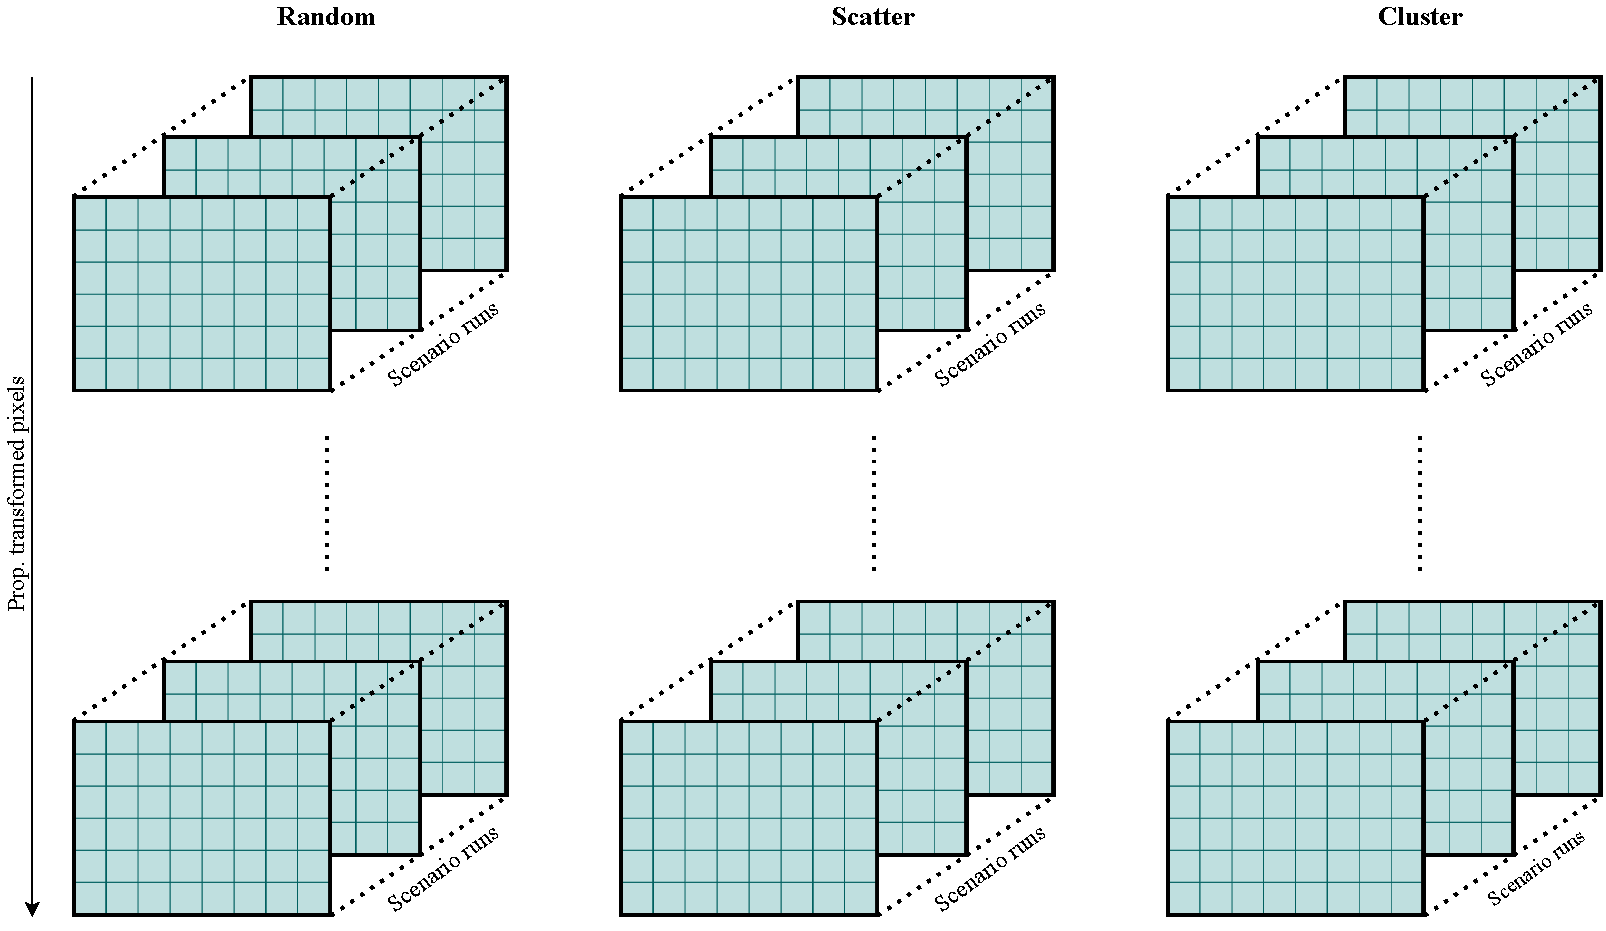
\includegraphics[width=\textwidth]{figures/scenario-scheme}
%   \caption{\label{fig:scenario-scheme} Scheme of the generated scenarios}
% \end{figure}


% \begin{figure}[ht]
%   \centering
%   \begin{tikzpicture}[x=(15:.5cm), y=(90:.5cm), z=(330:.5cm), >=stealth]
%     \draw (0, 0, 0) -- (0, 0, 10) (4, 0, 0) -- (4, 0, 10);
%     \foreach \z in {0, 5, 10} \foreach \x in {0,...,2}
%     \foreach \y [evaluate={\b=random(0, 1);}] in {0,...,3}
%     \filldraw [fill=white] (\x, \y, \z) -- (\x+1, \y, \z) -- (\x+1, \y+1, \z) --
%     (\x, \y+1, \z) -- cycle (\x+.5, \y+.5, \z) node [yslant=tan(15)] {\b};
%     \draw [dashed] (0, 4, 0) -- (0, 4, 10) (4, 4, 0) -- (4, 4, 10);
%     \draw [<->] (0, 4.5, 0)  -- (4, 4.5, 0)   node [near end, above left] {Approach};
%     \draw [->] (-.5, 4, 0)  -- (-.5, 0, 0)   node [midway, left] {Scenario run};
%     \draw [->] (4, 4.5, 10) -- (4, 4.5, 2.5) node [near end, above right] {Change prop.};
%   \end{tikzpicture}
  
%   \caption{\label{fig:label} }
% \end{figure}

% \subsubsection*{Quantifying the spatial patterns of tree canopy}
% with two main objectives. The first objective is to use the scenarios to explore the relationships between spatial patterns in both composition and configuration of trees and the distribution of air temperature simulated with the urban cooling model. The second objective is to inform policy-making.
% In order to explore the relationships between spatial pattern of the tree canopy in each scenario and its respective distribution of air temperature simulated with the urban cooling model.
% In order to quantify spatial pattern of the tree canopy of each scenario, a set of spatial metrics from landscape ecology \cite{o1988indices,mcgarigal2012fragstats} are computed for the pixels whose post-refinement LULC class has a high tree canopy cover.  % over a certain threshold.
For each scenario, the spatial pattern of the tree canopy is quantified by means of a set of spatial metrics from landscape ecology \cite{o1988indices,mcgarigal2012fragstats}, which are computed for the pixels whose post-refinement LULC class has a tree canopy cover over 75\% \footnote{Following the advice given by the directorate of resoures and natural heritage in the Canton of Vaud (DGE-DIRNA), the threshold over which a pixel is considered to have a high tree canopy cover has been set to 75\%, which corresponds to placing trees of a spheric crown with a 5~m radius spaced 10~m from one another so that they form a continuous canopy.}.
Based on other studies that explore the relationship between the spatial of tree canopy and UHIs, four spatial metrics have been chosen to quantify both the composition and oconfiguration of the tree canopy, which are listed in \autoref{tab:selected-metrics}. The proportion of landscape (PLAND) of pixels with high tree canopy cover serves to quantify the composition aspects, while the configuration is quantified by means of the mean patch size (MPS), edge density (ED) and the mean shape index (MSI) of patches of high tree canopy cover. The four metrics have been computed with the Python library PyLandStats \cite{bosch2019pylandstats}.

\begin{table}[!h]
  \begin{adjustwidth}{-.4\textwidth}{0cm} % Comment out/remove adjustwidth environment if table fits in text column.
    % \footnotesize % Font size can be changed to match table content. Recommend 10 pt.
    \caption{\label{tab:selected-metrics}Selected landscape metrics. A more thorough description can be found in the documentation of the software FRAGSTATS v4 \cite{mcgarigal2012fragstats}}
    \renewcommand{\arraystretch}{1.5} % vertical spacing
    \begin{center}
      \begin{tabular}{p{.15\textwidth} p{.4\textwidth} p{.76\textwidth}} 
        \toprule
        \textbf{Category} & \textbf{Metric name} & \textbf{Description} \\
        \midrule
        Composition & Percentage of landscape (PLAND) & Percentage of landscape, in terms of area, occupied by pixels with high tree canopy cover \\
        Configuration & Mean patch area (AREA\_MN) & Average size (in hectares) of the patches formed by pixels with high tree canopy cover \\
        & Mean shape index (SHAPE\_MN) & Average shape index of the patches formed by pixels with high tree canopy cover \\
        & Edge density (ED) & Sum of the lengths of all edge segments between pixels with high tree canopy cover an other pixels, per area unit (in m/hectare) \\    
        \bottomrule  
      \end{tabular}
    \end{center}
  \end{adjustwidth}
\end{table}

% \subsubsection*{Simulation of urban greening by randomly increasing the proportion of tree cover}
% With the aim of evaluating the effect of the proportion of tree cover on air temperature, a set of scenarios is generated by transforming a 25, 50, 75 and 100\% of the pixels where the tree canopy cover can be increased.
% For each of the aforementioned percentages, a number scenario runs will be generated by randomly sampling from the candidate pixels until the desired proportion of changed pixels is matched. Therefore, the temperature maps for each of the percentage of changed pixels will be computed by averaging the respective simulated runs.
% After observing little variability among the simulation runs, the number of scenario runs has been set to 10.

% \subsubsection*{Simulation of distinct urban greening approaches by clustering and scattering the tree canopy}

% % To expore the relationship between
% In order to obtain a greater variety of spatial patterns of tree canopy cover and further explore the relationship between the spatial configuration of tree canopy and UHIs, two additional sets of scenarios will be generated.
% % Like the first set of scenarios described above, these two additional sets are also produced by transforming a 25, 50, 75 and 100\% of the pixels where the tree canopy can be increased.
% % Nevertheless, in these two sets the transformed pixels are not randomly sampled but selected according to the number of pixels with high tree canopy cover (i.e., > 75\%) found in their Moore neighborhood. Therefore,
% In these sets of scenarios, the transformed pixels are not randomly sampled but selected according to the number of pixels with high tree canopy cover (i.e., greater than 75\%) found in their Moore neighborhood.
% Therefore, the first set of scenarios pixels with higher number of high tree canopy cover neighbors are transformed first, which intends to spatially cluster pixels of high tree canopy cover. Conversely, the second set of scenarios intends to spatially scatter pixels of high tree canopy cover by giving precedence to pixels with lower number of high tree canopy neighbors.
% To explore the difference between the two approaches with more detail, these two sets of scenarios will be produced by transforming a 12.5, 25, 37.5, 50, 62.5, 75 and 87.5 of the pixels where the tree canopy can be increased.
% The scenario where all the candidate pixels, i.e., 100\%, are transformed is excluded here because under such such circumstances the clustering or scattering criteria to select the pixels does not have any effect.
% Like the previous set of scenarios, the temperature maps will be computed by averaging the results of 10 simulation funs for each configuration, i.e., combination of proportion of changed pixels and spatial approach of either clustering or scattering the transformed pixels. This results in a total of 140 scenarios, where 70 correspond to the clustering approach and the other 70 to the scattering approach.


\section*{Results}

% \subsection{Performance of the urban cooling model}



% \subsection{Relationship between the spatial pattern of tree canopy on urban heat mitigation}

% The coefficients estimated with the OLS regression are listed in \autoref{tab:selected-metrics}. Although the values of the Moran I \cite{moran1950notes} suggest a strong spatial autocorrelation, the use of a spatial regression model does not improve the coefficient of determination nor change the sign of any coefficient at any scale (see \ref{sec:spatial-relationships}). Therefore, the remainder of the article will only consider the OLS regression.
% In line with the results of Zhou et al. \cite{zhou2017effects}, the coeffient of determination increases with the scale, whereas the Moran I and the Akaike information criterion (AIC) \cite{akaike1973information} decrease, suggesting that the linear regression model performs better at larger scales.

% \begin{table}
%   \caption{\label{tab:ols-regression} Results of the OLS regression.}
%   \scriptsize % Font size can be changed to match table content. Recommend 10 pt.
%   \begin{center}
%     \begin{tabular}{ p{.065\textwidth} p{.11\textwidth} p{.11\textwidth} p{.11\textwidth} p{.11\textwidth} p{.11\textwidth} p{.055\textwidth} p{.07\textwidth} p{.07\textwidth} }
%       \toprule
%       Scale & PLAND & AREA\_MN & SHAPE\_MN & ED & DIST & R$^2$ & Moran & AIC\\
%       \midrule
%       120~m & -0.013741** & 0.375819** & -0.169583** & 0.000688** & -0.000119** & 0.414 & 0.872** & 9472.641 \\
%       & \textbf{-0.353207} & \textbf{0.130888} & \textbf{-0.055450} & \textbf{0.102536} & \textbf{-0.347371} \\
%       360~m & -0.016759** & 0.111463** & -0.365982** & 0.001481** & -0.000113** & 0.459 & 0.796** & 1335.884 \\
%       & \textbf{-0.340134} & \textbf{0.166164} & \textbf{-0.145221} & \textbf{0.175597} & \textbf{-0.337706} \\      
%       600~m & -0.023965** & 0.265071** & -0.635437** & 0.002251** & -0.000105** & 0.491 & 0.678** & 501.365 \\
%       & \textbf{-0.436498} & \textbf{0.248360} & \textbf{-0.202908} & \textbf{0.240449} & \textbf{-0.313095} \\
%       840~m & -0.029608** & 0.295937* & -0.529756** & 0.003047** & -0.000098** & 0.533 & 0.572** & 255.563 \\
%       & \textbf{-0.489575} & \textbf{0.180218} & \textbf{-0.161129} & \textbf{0.291127} & \textbf{-0.296891} \\
%       1080~m & -0.023499** & 0.233338 & -1.413028** & 0.002752** & -0.000106** & 0.564 & 0.486** & 154.011 \\
%       & \textbf{-0.360574} & \textbf{0.139134} & \textbf{-0.190122} & \textbf{0.233989} & \textbf{-0.311524} \\      
%       \bottomrule
%     \end{tabular}
%   \end{center}
%   ** $P < 0.01$, * $P < 0.05$ (2-tailed)
% \end{table}

% The standardized coefficients suggest that proportion of tree canopy cover is the feature that has most heat mitigation effect at all scales, followed by the distance to the city center. Among the configuration metrics, the edge density has the most significant effect on air temperature, which suggest that a more edgy tree canopy pattern contributes to higher temperatures. A similar positive effect is observed for the mean patch size, nonetheless it becomes less significant at larger scales. Finally, the mean shape index has a negative effect on air temperature which indicates that more irregular tree canopy patches contribute to greater heat mitigation.

% % \begin{table}
% %   \footnotesize % Font size can be changed to match table content. Recommend 10 pt.
% %   \begin{center}
% %     \begin{tabular}{ p{.07\textwidth} p{.11\textwidth} p{.11\textwidth} p{.11\textwidth} p{.11\textwidth} p{.11\textwidth} p{.07\textwidth} p{.08\textwidth} }
% %       \toprule
% %       Scale & PLAND & AREA\_MN & SHAPE\_MN & ED & DIST & R$^2$ & AIC\\
% %       \midrule
% %       120~m & -0.027518 & 1.075121 & -0.340077 & 0.001006 & -0.000118 & 0.381 & inf \\
% %       360~m & -0.020581 & 0.088502 & -0.206741 & 0.001568 & -0.000112 & 0.449 & 1664.495 \\
% %       600~m & -0.003655 & 0.033896 & -0.150886 & 0.000321 & -0.000131 & 0.357 & -248.053 \\
% %       840~m & -0.007555 & 0.073376 & -0.163887 & 0.000450 & -0.000123 & 0.411 & -39.204 \\
% %       1080~m & -0.014000 & 0.146802 & -0.678353 & 0.000938 & -0.000103 & 0.535 & 114.427 \\
% %       \bottomrule
% %     \end{tabular}
% %     \caption{\label{tab:spatial-regression} Results of the spatial regression.}
% %   \end{center}
% % \end{table}

% The correlation coefficients for the Pearson correlation and the partial correlation analysis are listed in \autoref{tab:correlation-coefficients}. The distance to the city center is the feature that is most negatively correlated to air temperature, and its effect increases when controlling for the proportion of tree cover. Each of the configuration metrics shows a distinctive response to the partial correlation analysis. The mean patch size becomes shows a clear decrease on its negative influence on air temperature when controlling for the proportion of tree cover, even losing the $P < 0.05$ significance level at the largest scale. In sharp contrast, the mean shape index increases its negative effect on air temperature, whereas the edge density changes from a positive correlation with air temperature to a negative effect with a similar level of significance. Contrarily to the OLS regression above, the results of the partial correlation suggest that increasing the edges between tree and non-tree pixels contributes to urban heat mitigation. On the other hand, when controlling for the effects of the configuration metrics, the proportion of tree cover shows an increase on its negative effect on air temperature. Finally, with very few exceptions, the correlation coefficients increase with the scale. 

% \begin{table}
%   \caption{\label{tab:correlation-coefficients} Correlation coefficients. The bold rows show the coefficients of the partial correlation analysis.}
%   \footnotesize % Font size can be changed to match table content. Recommend 10 pt.
%   \begin{center}
%     \begin{tabular}{ p{.075\textwidth} p{.13\textwidth} p{.13\textwidth} p{.13\textwidth} p{.13\textwidth} p{.13\textwidth}}
%       \toprule
%       Scale & PLAND & AREA\_MN & SHAPE\_MN & ED & DIST \\
%       \midrule
%       120~m & -0.335816** & -0.326044** & -0.203751** & -0.021708 & -0.542007** \\
%       & \textbf{-0.201833}** & \textbf{-0.053347}** & \textbf{-0.140807}** & \textbf{-0.024849}* & \textbf{-0.575068}** \\
%       360~m & -0.304223** & -0.230111** & -0.293065** & 0.090014* & -0.545207** \\
%       & \textbf{-0.353835}** & \textbf{-0.038458} & \textbf{-0.299635}** & \textbf{-0.145022}** & \textbf{-0.595347}** \\      
%       600~m & -0.340180** & -0.334422** & -0.343264** & 0.111613* & -0.535269**  \\
%       & \textbf{-0.398365}** & \textbf{-0.129310}* & \textbf{-0.374636}** & \textbf{-0.177379}** & \textbf{-0.593629}** \\
%       840~m & -0.368275** & -0.392994* & -0.343015** & 0.114636 & -0.544322** \\
%       & \textbf{-0.428976}** & \textbf{-0.180682}* & \textbf{-0.457676}** & \textbf{-0.173731}* & \textbf{-0.606605}** \\
%       1080~m & -0.342848** & -0.346385 & -0.354632** & 0.236678** & -0.569577**  \\
%       & \textbf{-0.428303}** & \textbf{-0.177690} & \textbf{-0.484208}** & \textbf{-0.215491}* & \textbf{-0.650891}** \\      
%       \bottomrule
%     \end{tabular}
%   \end{center}
%   ** $P < 0.01$, * $P < 0.05$ (2-tailed)
% \end{table}


% \subsection{Evaluation of the greening scenarios}

\subsection*{Proportion of transformed pixels by their original LULC class}

The relationship between the number of transformed candidate pixels by their original LULC class and the overall proportion of transformed candidate pixels is shown in \autoref{fig:scenario-lulc-barplot}.
Changing a 25, 50, 75 and 100\% of the candidate pixels corresponds to a total number of pixels changed of 118880, 237760, 356640 and 475520, which account for a total area of 1188.8, 2377.6, 3566.4 and 4755.2 hectares respectively.
In the latter case, i.e., increasing the tree canopy in all the possible pixels, 61.50\% of the pixels correspond to the ``garden'' LULC class, followed by ``road, path'', ``building'', ``other impervious'', (18.01, 10.81 and 7.69\%, respectively). Finally, the LULC classes of ``sidewalk'' and ``traffic island'' constitute only 1.67 and 0.3\% of the  pixels where the tree canopy can be increased.
% changing a 25, 50, 75 and 100\% of the potential pixels corresponds to a total number of pixels changed of 118880, 237760, 356640 and 475520 respectively.
% On average over all the simulation runs and sampling approaches,
The differences when considering the sampling approaches separately are small relative to the total number of transformed candidate pixels.
The largest differences between sampling approaches can be noted in the number of transformed pixels that originally belong to the ``garden'' class.
% which the clustering approach consistently transforms a larger share of pixels of the ``garden''
When transforming 25, 50 and 75\% of the candidate pixels, clustering respectively transforms (on average among the simulation runs) a 0.90, 0.38 and 0.12\% more garden pixels than random sampling, and 1.28, 0.76 and 0.43\% more garden pixels than the scattering approach (\autoref{fig:scenario-lulc-barplot-comparison}). 

% CI are of course, inexistent when changing all the possible pixels
% The confidence intervals are very small for all the proportions of pixels changed, which reflects the constraints imposed by the existing urban fabric.

\begin{figure}[H]
  \centering
  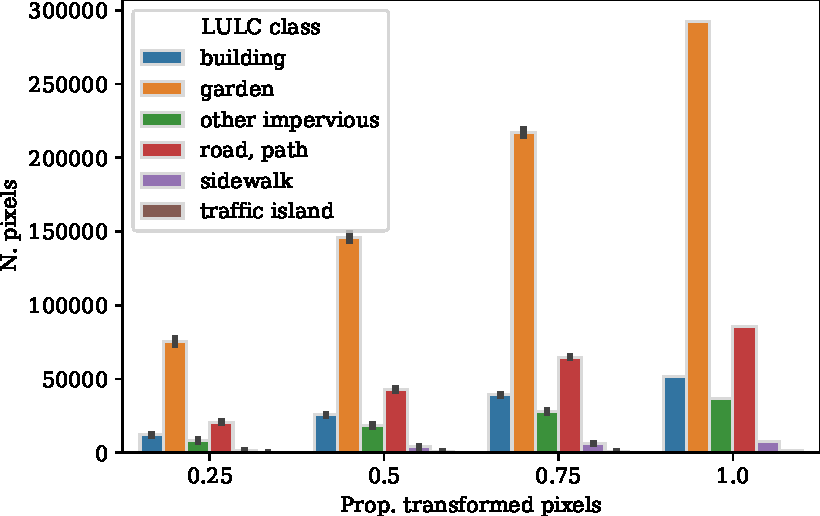
\includegraphics[width=.6\textwidth]{figures/scenario-lulc-barplot}%
  \caption{\label{fig:scenario-lulc-barplot} Number of transformed pixels by its original LULC class for an overall proportion of transformed pixels of 25, 50, 75 and 100\%. The lines at the top of the bars represent the 95\% confidence intervals. The bar heights and the confidence intervals are computed out of all the simulation runs and sampling approaches. See the Jupyter Notebook at \hyperref[sec:si-scenarios]{section S2.1} for the detailed numbers of the figure.}
\end{figure}

\begin{figure}[H]
  \begin{adjustwidth}{-.4\textwidth}{0cm}  
    \centering
    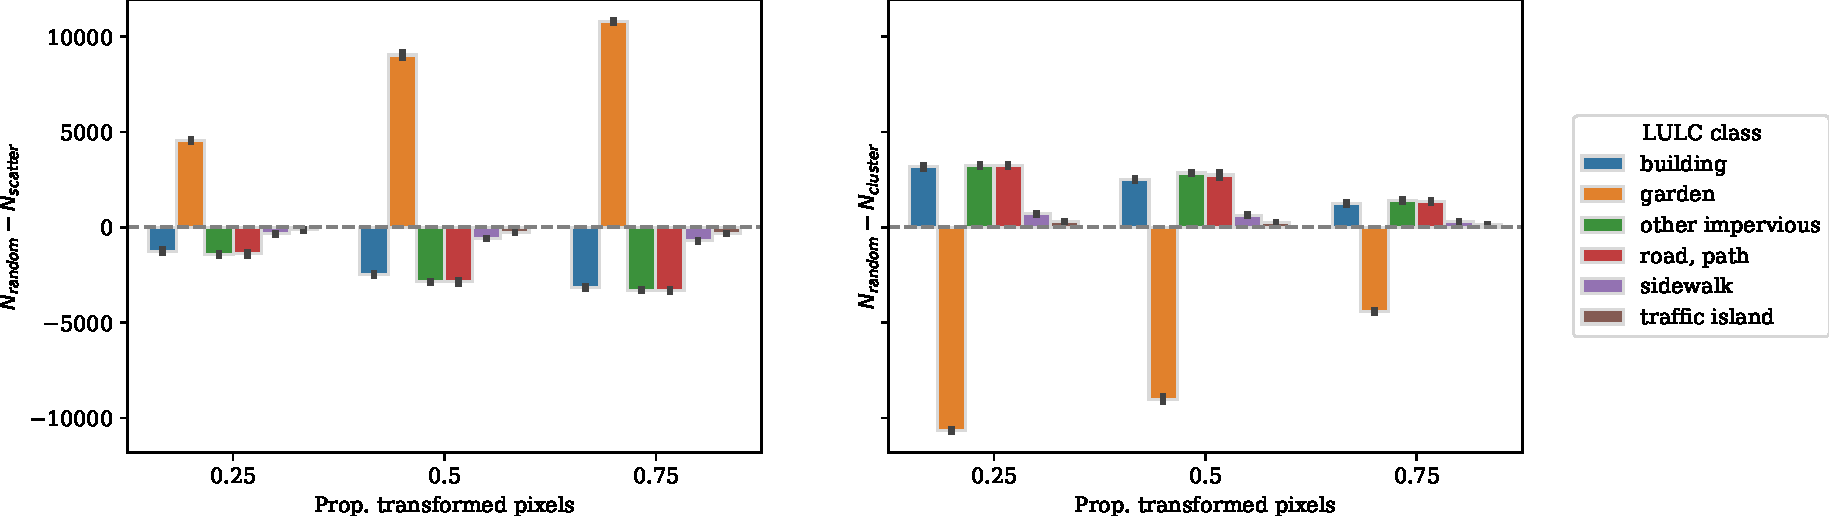
\includegraphics[width=\linewidth]{figures/scenario-lulc-barplot-comparison}
    \caption{\label{fig:scenario-lulc-barplot-comparison}
      Comparison of between the number of transformed pixels by its original LULC class with the random sampling approach and the scattering ($N_{random} - N_{scatter}$, left subplot) and the clustering ($N_{random} - N_{cluster}$, right subplot) selection approaches, for an overall proportion of transformed pixels of 25, 50 and 75\%.
      The lines at the top of the bars represent the 95\% confidence intervals. The bar heights and the confidence intervals are computed out of all the simulation runs. See the Jupyter Notebook at \hyperref[sec:si-scenarios]{section S2.1} for the detailed numbers of the figure.}
  \end{adjustwidth}
\end{figure}


\subsection*{Simulated LULC, temperature and heat mitigation maps}

% A set scenario LULC maps generated with increasing proportion of pixels changed to its corresponding LULC code with high tree canopy cover, its corresponding simulated air temperatuers and heat mitigation are shown in \autoref{fig:scenarios-prop} (see \ref{sec:scenarios-prop}).
% The maps for four scenarios generated by changing an increasing proportion of pixels to its corresponding LULC code with high tree canopy cover are shown in \autoref{fig:scenario-maps}.
The LULC, temperature and heat mitigation maps for the scenarios generated by transforming a 25, 50, 75 and 100\% of the candidate pixels are shown in \autoref{fig:scenario-maps}.
% \begin{figure}
%   \begin{subfigure}{\textwidth}
%     \centering
%     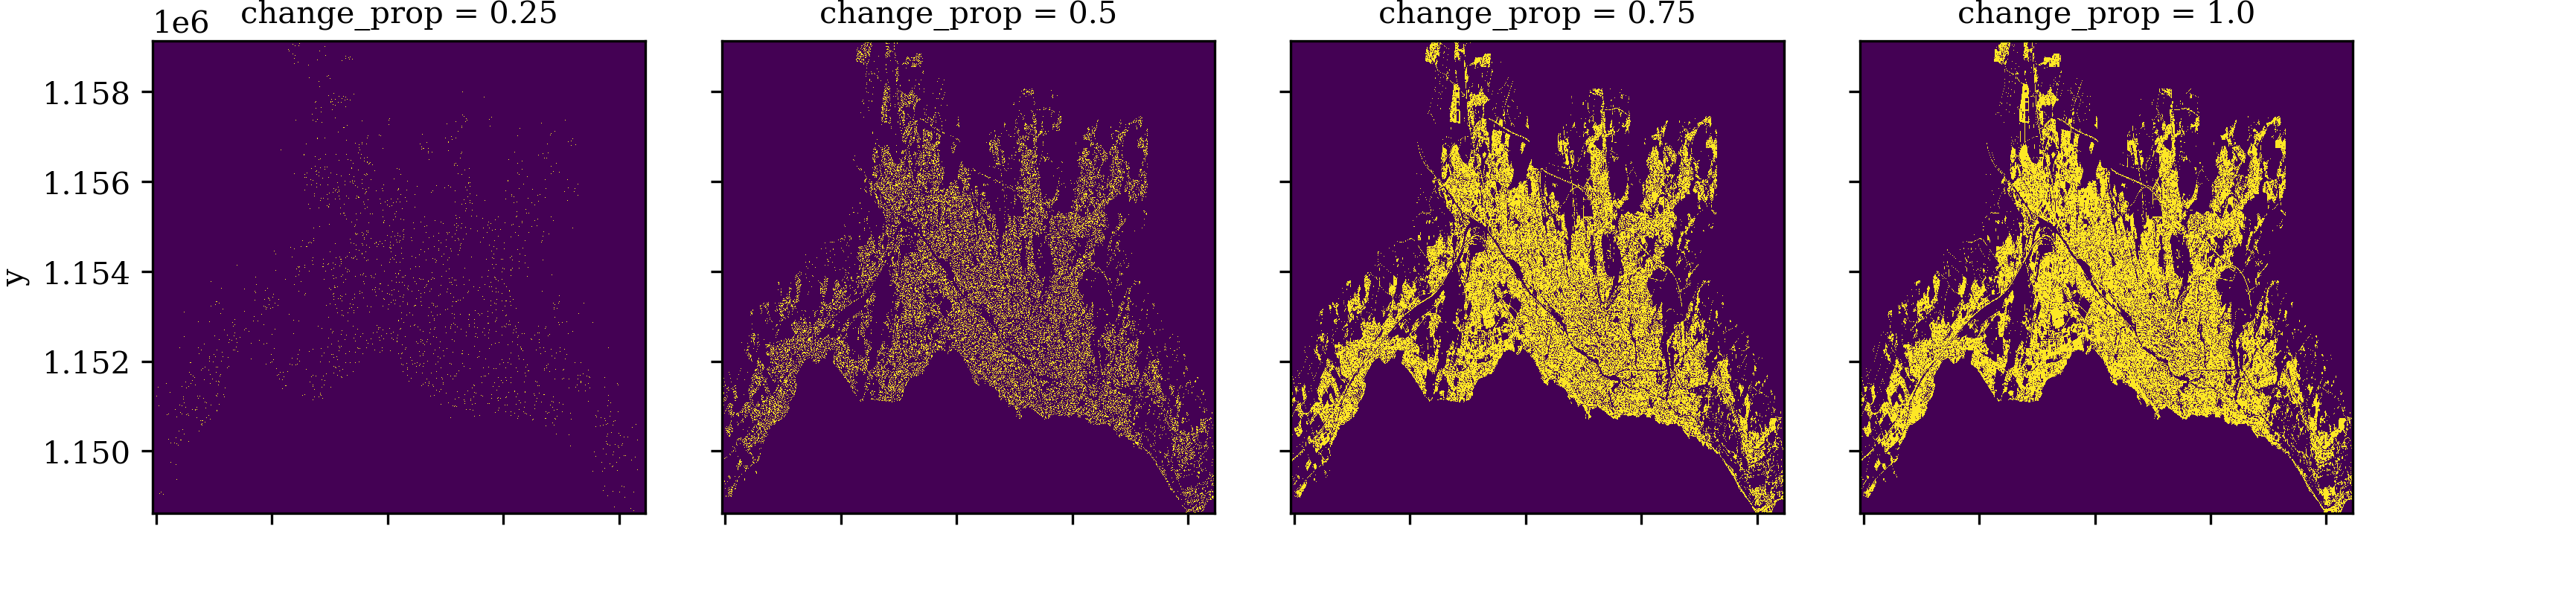
\includegraphics[width=\textwidth]{figures/scenarios-prop-lulc.png}
%   \end{subfigure}
%   \begin{subfigure}{\textwidth}
%     \centering    
%     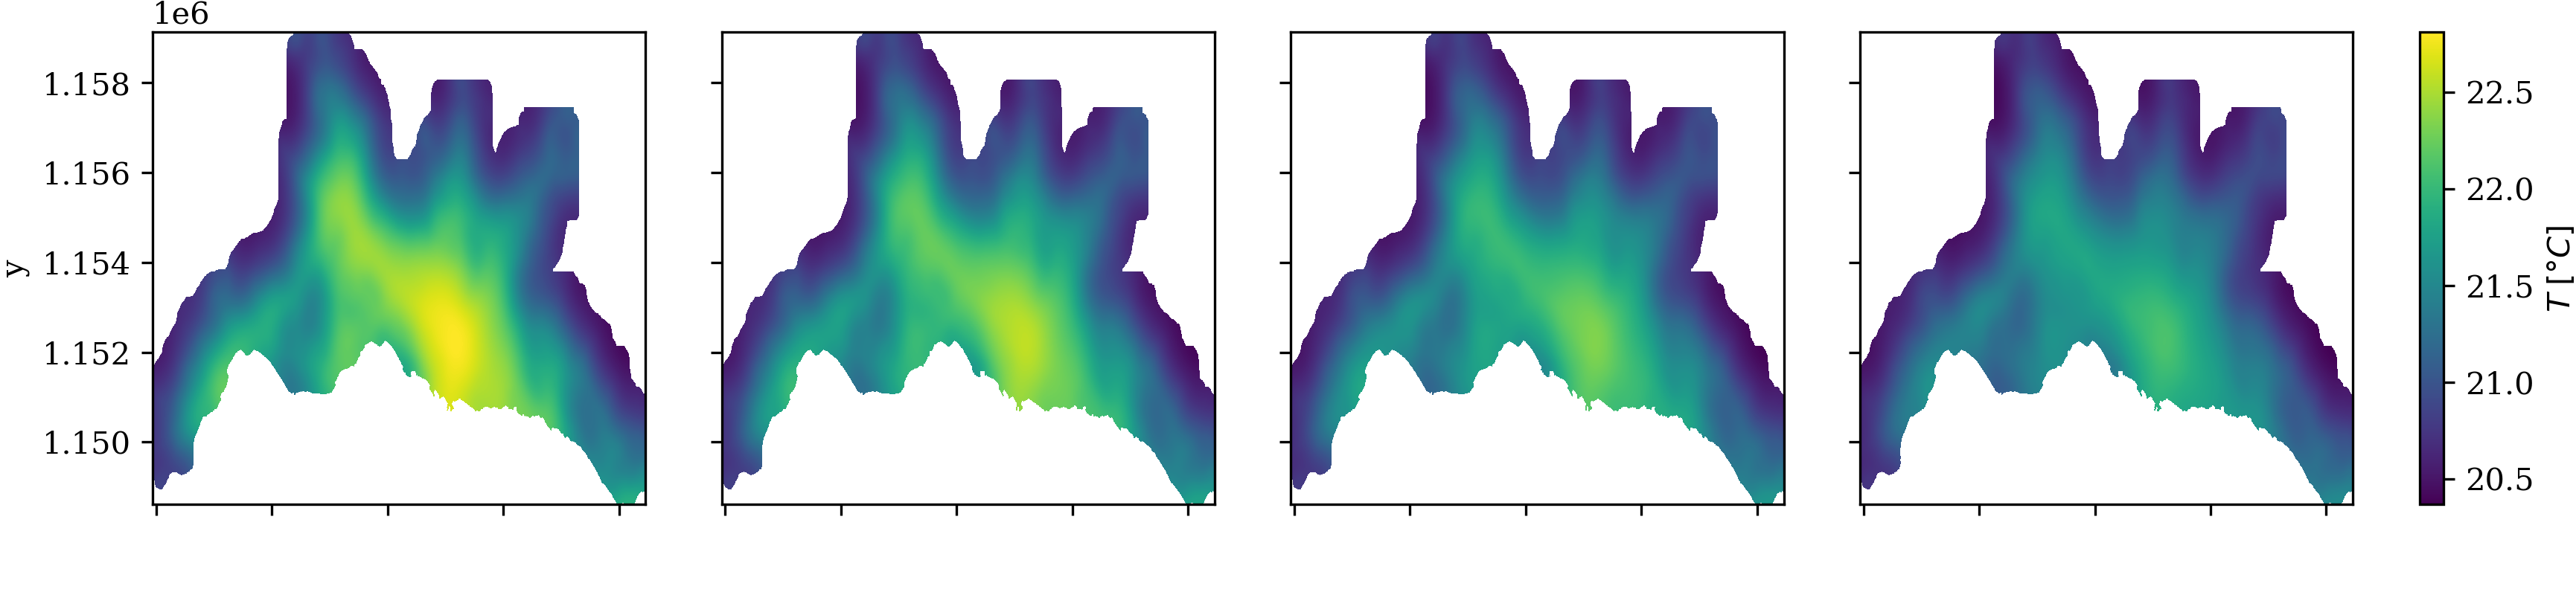
\includegraphics[width=\textwidth]{figures/scenarios-prop-T.png}  
%   \end{subfigure}
%   \begin{subfigure}{\textwidth}
%     \centering    
%     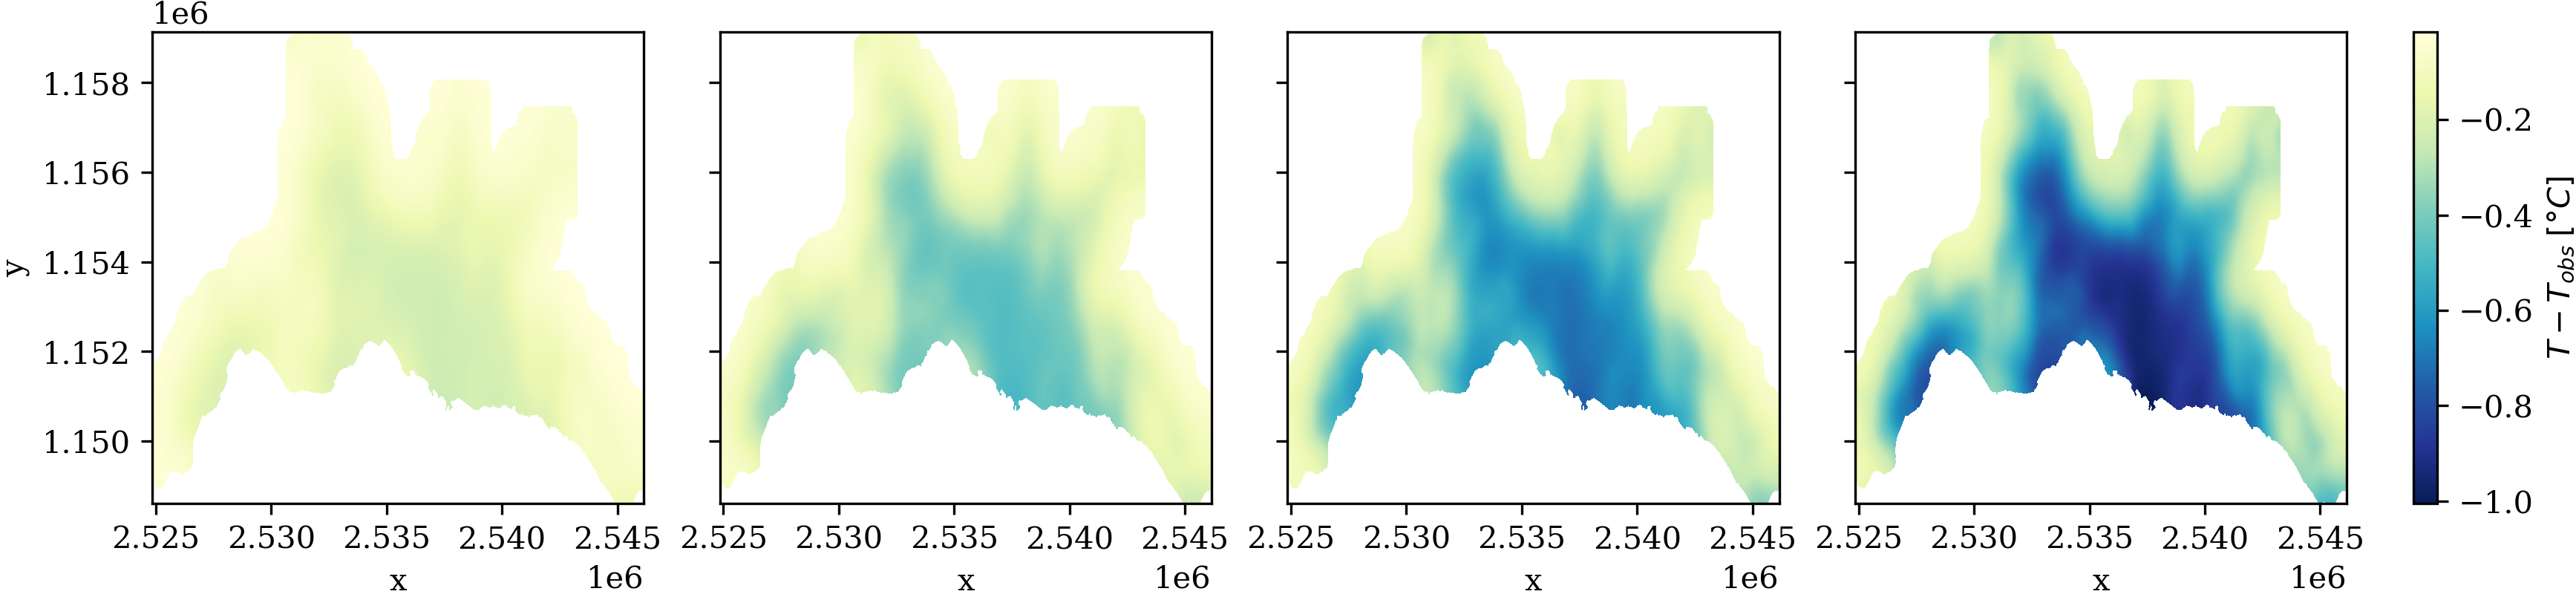
\includegraphics[width=\textwidth]{figures/scenarios-prop-mitigation.png}
%   \end{subfigure}
%   \caption{\label{fig:scenarios-prop} Scenario raster maps with an increasing (from left to right) proportion of the pixels changed to its corresponding LULC code with high tree canopy cover. The rows respectively feature the pixels where the LULC is changed (top), the simulated air temperature (middle) and the simulated heat mitigation (bottom).}
% \end{figure}
\begin{figure}
  \begin{adjustwidth}{-.4\textwidth}{0cm}
    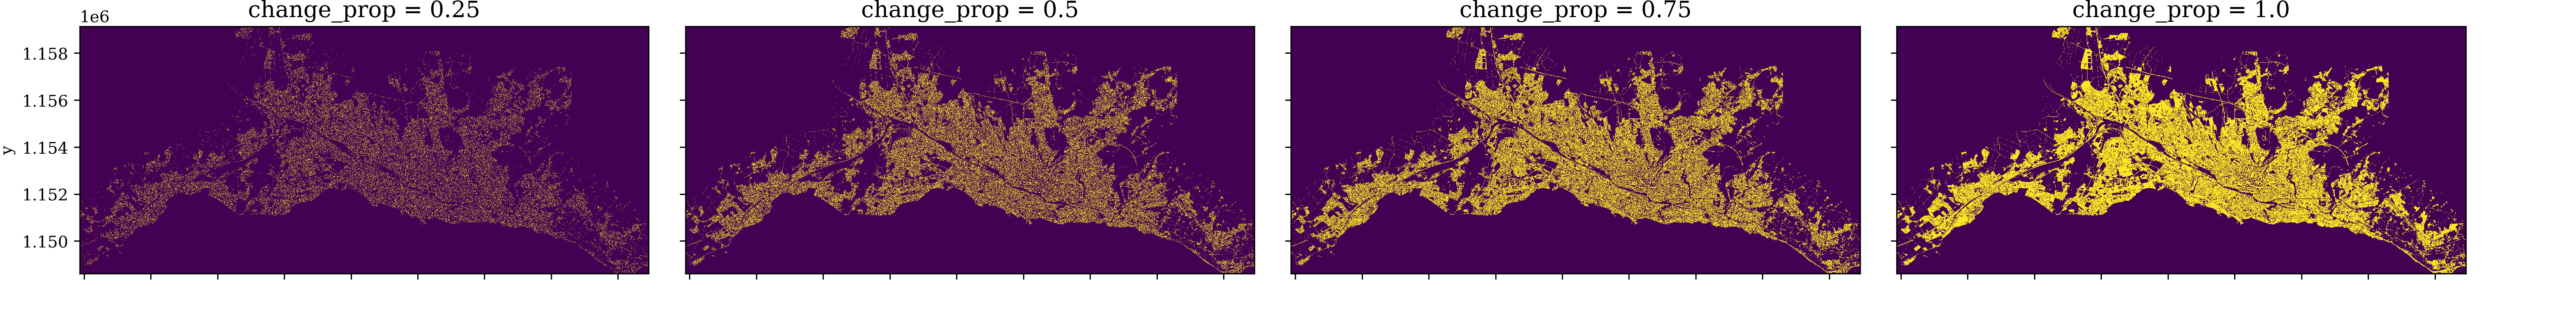
\includegraphics[width=\linewidth]{figures/scenario-lulc-maps.png}
    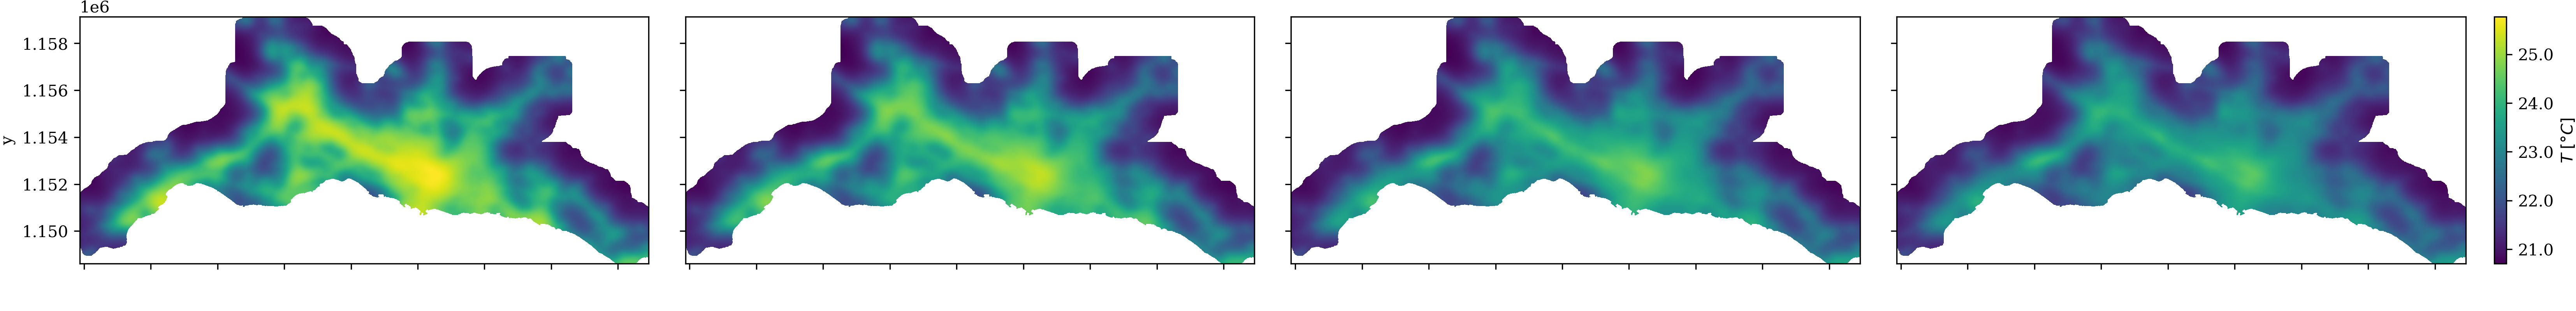
\includegraphics[width=\linewidth]{figures/scenario-T-maps.png}
    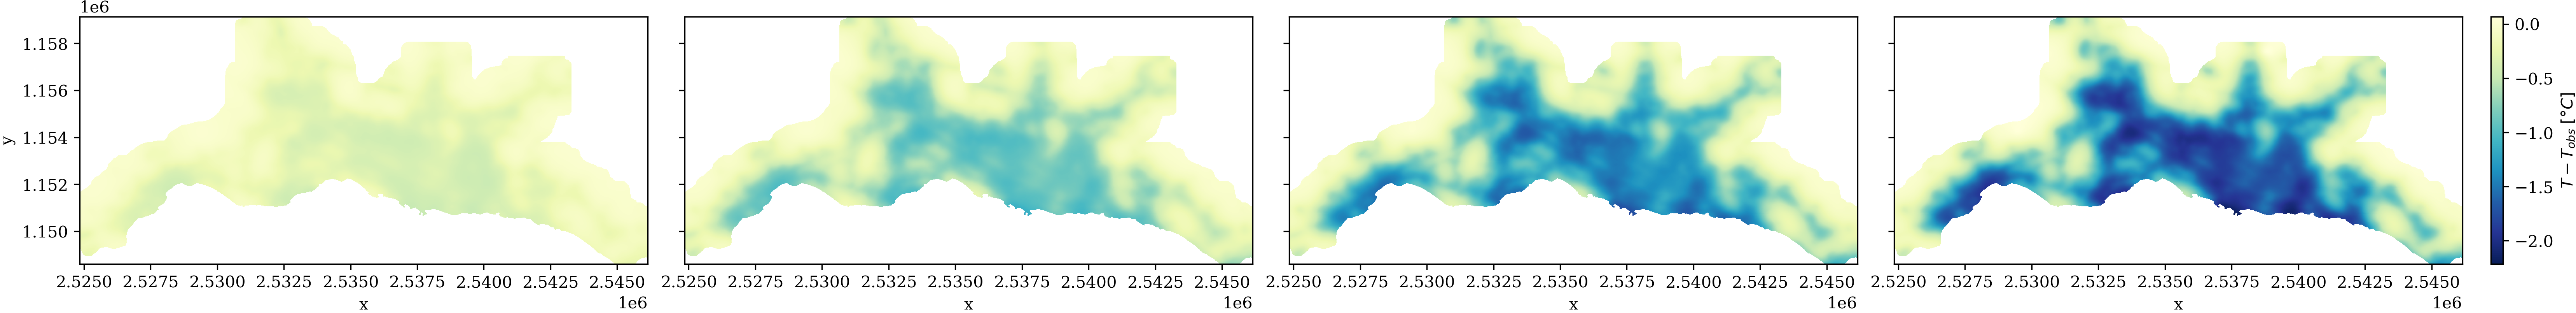
\includegraphics[width=\linewidth]{figures/scenario-heat-mitigation-maps.png}
    % \begin{subfigure}{\linewidth}
    %   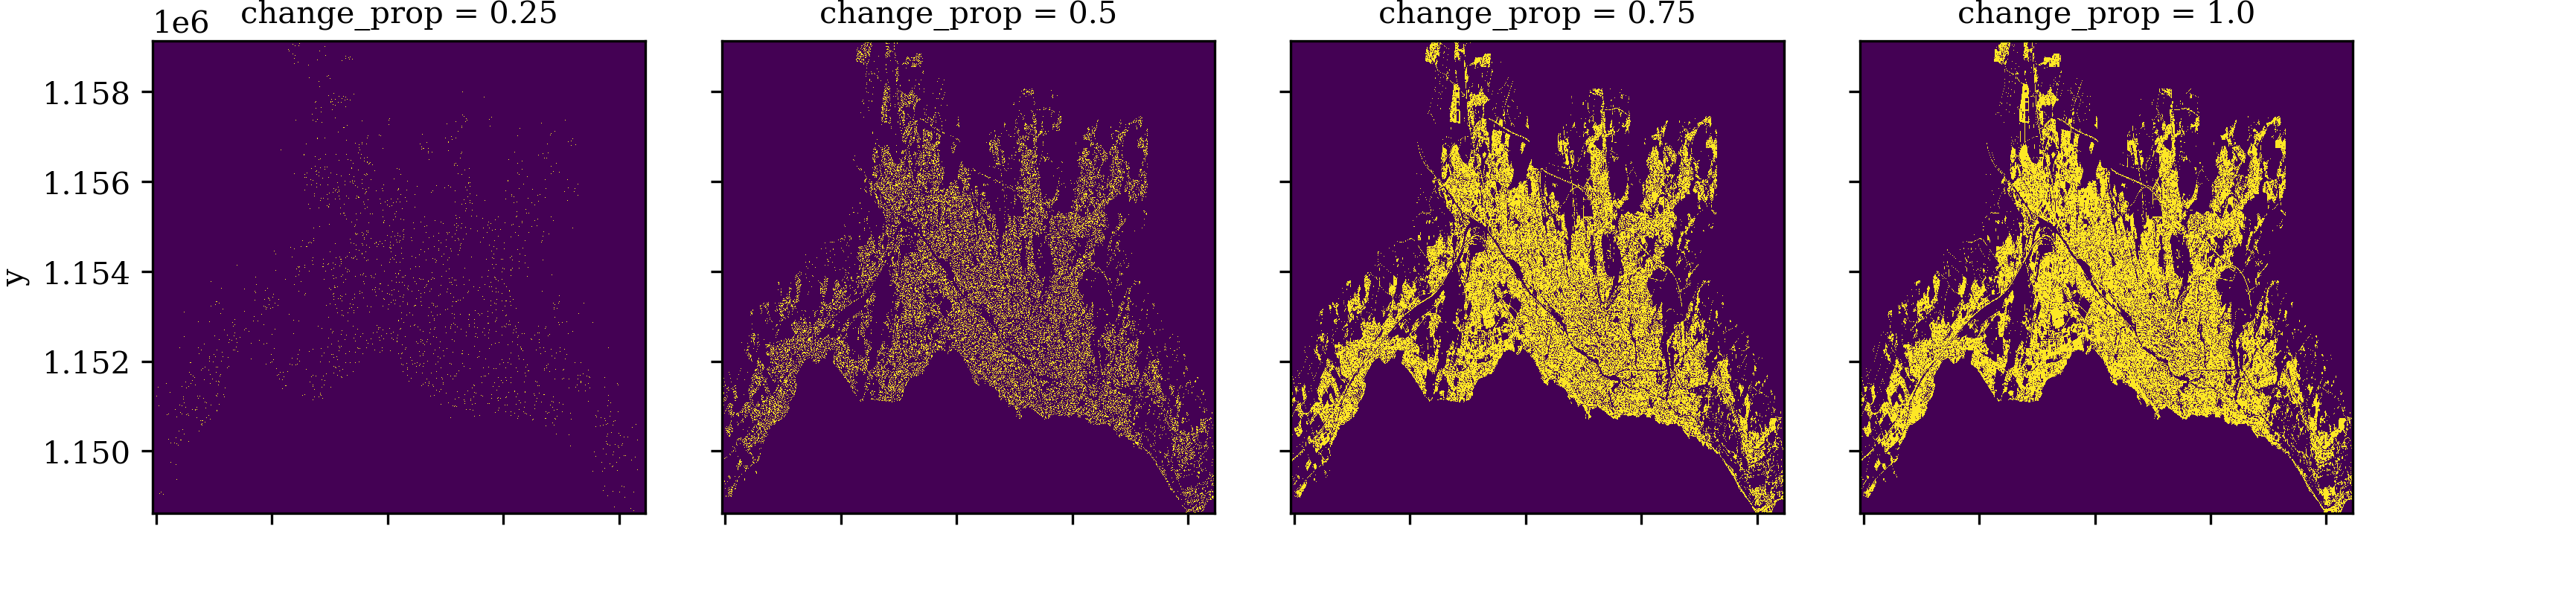
\includegraphics[width=\textwidth]{figures/scenarios-prop-lulc.png}
    % \end{subfigure}
    % \begin{subfigure}{\linewidth}
    %   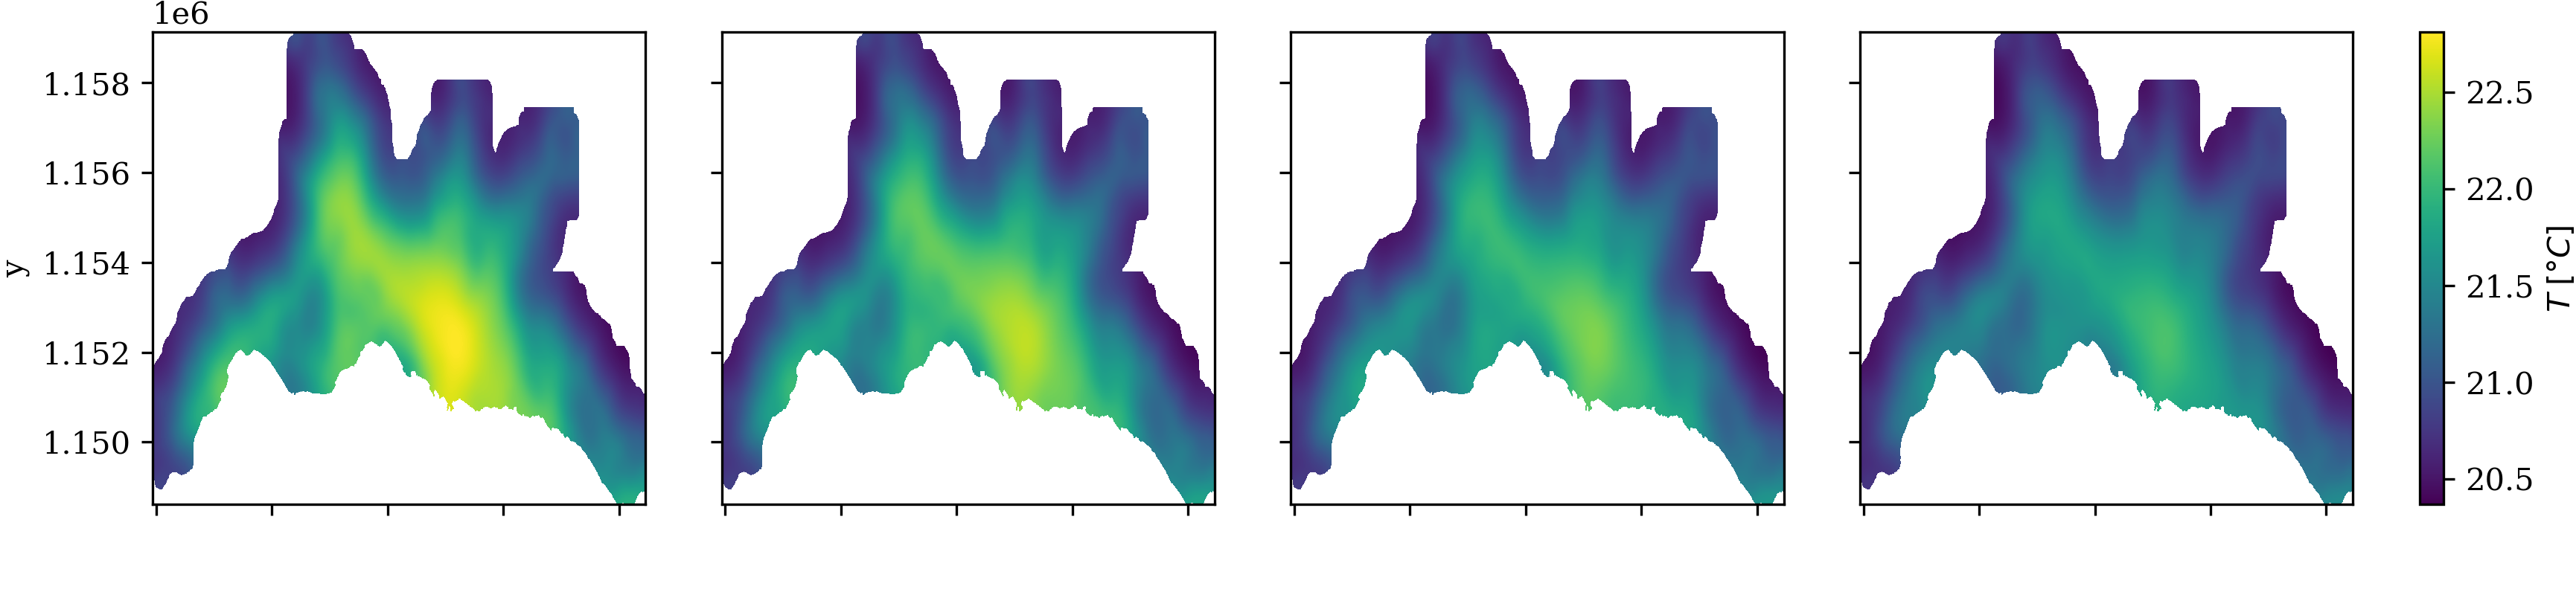
\includegraphics[width=\textwidth]{figures/scenarios-prop-T.png}  
    % \end{subfigure}
    % \begin{subfigure}{\linewidth}
    %   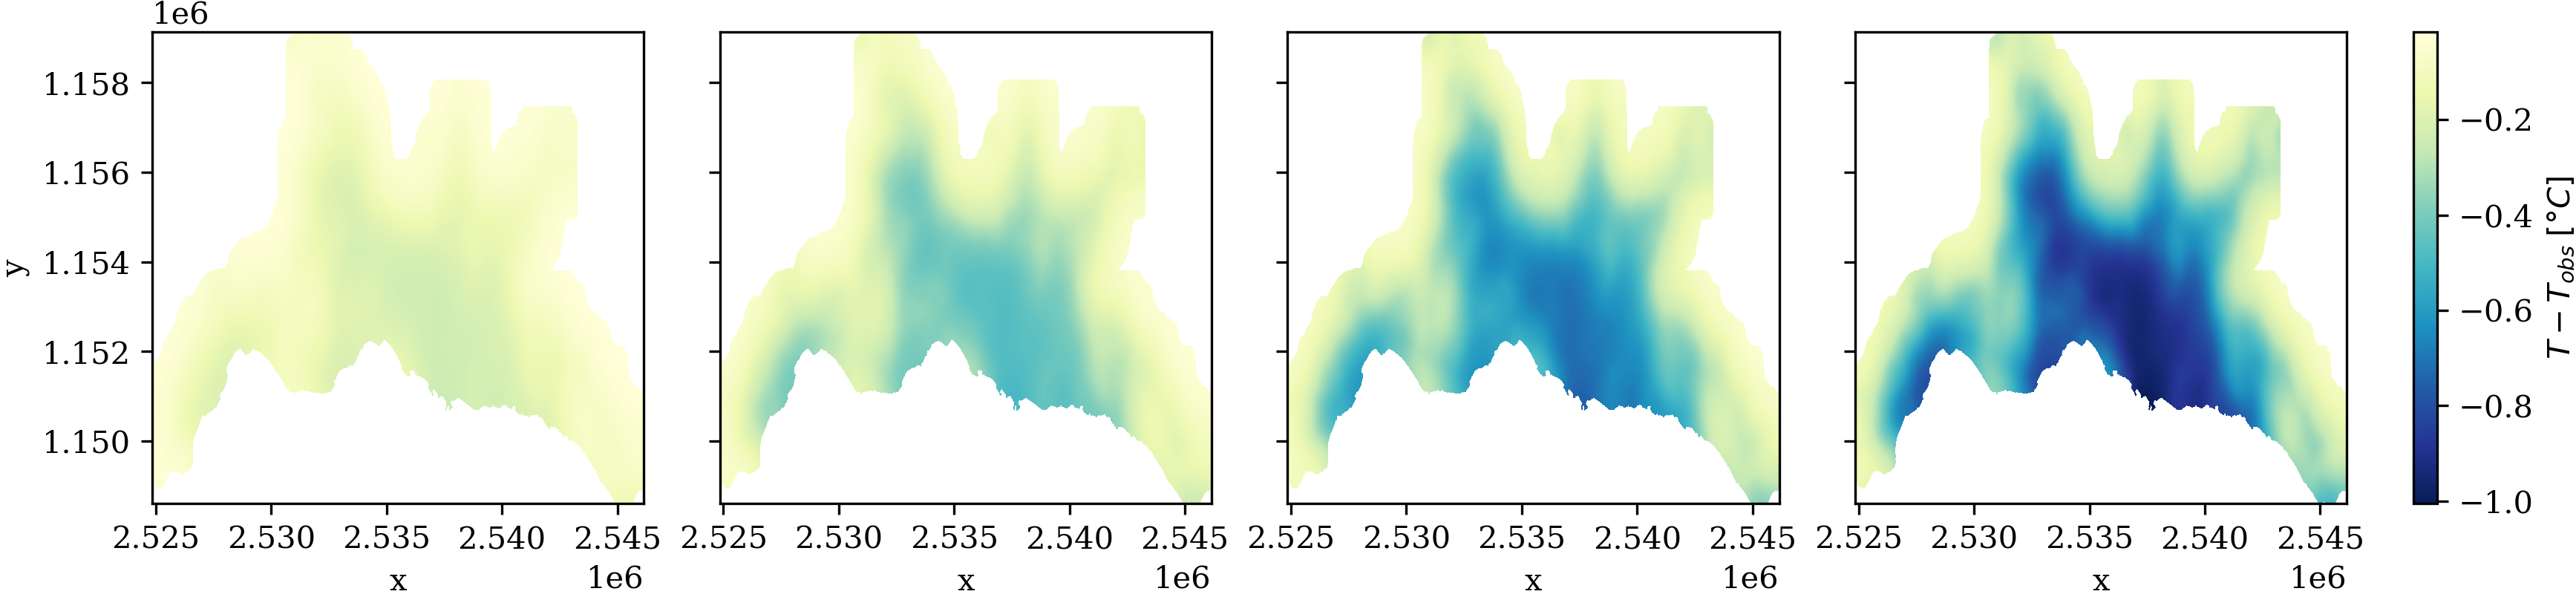
\includegraphics[width=\textwidth]{figures/scenarios-prop-mitigation.png}
    % \end{subfigure}
    % \captionsetup{width=\linewidth, margin={0cm,-.4\textwidth}}
    \caption{\label{fig:scenario-maps} Simulated LULC (top), temperature (middle) and heat mitigation (bottom) maps by transforming a 25, 50, 75 and 100\% of the candidate pixels to its corresponding LULC code with high tree canopy cover. The pixel values of each map are aggregated out of all the sampling approaches and simulation runs, i.e., the LULC maps show the mode, whereas the temperature and heat mitigation maps show the average. The axes tick labels display the Swiss CH1903+/LV95 coordinates. See the Jupyter Notebook at \hyperref[sec:si-scenarios]{section S2.1} for the detailed numbers of the figure.}
  \end{adjustwidth}
\end{figure}
When changing 25, 50, 75 and 100\% of the candidate pixels, the maximum temperature $T$ for the reference date, i.e., 26.05$\degree C$, is progressively reduced to 25.77, 25.30, 24.82 and 24.49$\degree C$ respectively, while the magnitude of maximum heat mitigation ($T - T_{obs}$) increases from 0.49, 1.17, 1.81 and 2.22$\degree C$ respectively.
The largest heat mitigation magnitudes occur in the most urbanized parts, which are located along the main transportation axes.
The relationship between the proportion of candidate pixels transformed and the simulated distribution of air temperature can be approximated as a linear relationship with a negative slope (see \autoref{fig:si-scenario-T-regplot} and \autoref{fig:si-scenario-T-hists} for more details about this relationship).
% The strength of such a fit suggests that the constraints on the urban heat mitigation imposed by the existing urban fabric .


\subsection*{Spatial patterns of tree canopy cover}

The relationships between the landscape metrics of each scenario run and the corresponding simulated average temperature $\overline{T}$ (over all the pixels) are displayed in \autoref{fig:scenario-metrics}.
\begin{figure}
  \begin{adjustwidth}{-.4\textwidth}{0cm}  
    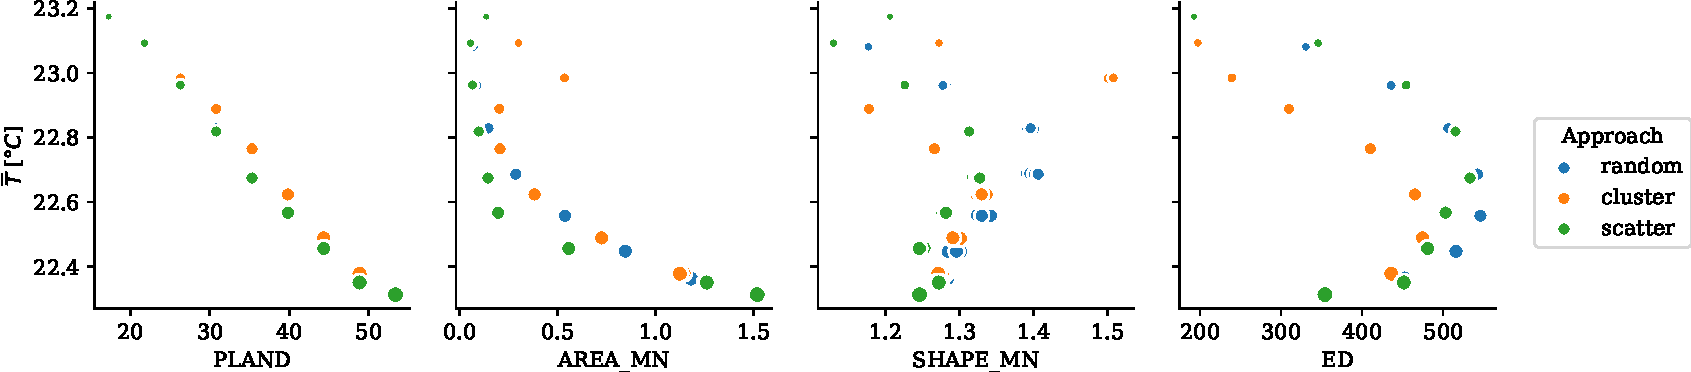
\includegraphics[width=.99\linewidth]{figures/scenario-metrics}
    % \captionsetup{width=\linewidth, margin={0cm,-.4\textwidth}}
    \caption{\label{fig:scenario-metrics} Relationship between landscape metrics and the simulated average temperature $\overline{T}$ for each scenario run, colored to distinguish the sampling approaches. See the Jupyter Notebook at \hyperref[sec:si-scenario-metrics]{section S2.2} for the detailed numbers of the figure.}
  \end{adjustwidth}
\end{figure}
% The values of PLAND, which are directly related to the proportion of tranformed candidate pixesl
The proportion of landscape (PLAND) occupied by pixels with high tree canopy cover range from 17.26 to 53.37\%. As a composition metric, PLAND is directly related to the proportion of transformed candidate pixels, and the extreme values of the PLAND range correspond to transforming 0 and 100\% of the candidate pixels respectively.
The relationship between PLAND and the average simulated temperature of each scenario $\overline{T}$ shows a sharp monotonic decrease. However, for the same PLAND values, clustering the transformed pixels to other pixels with high tree canopy cover consistently leads to higher $\overline{T}$ than scattering or randomly sampling --- the latter approaches show almost indistinguishable PLAND and $\overline{T}$ relationship.
% With the exception of the mean shape index,

Regarding the configuration metrics, the values of the mean patch area (AREA\_MN) show that the clustering and random sampling approaches lead to larger patches of high tree canopy cover than the scattering approach.
When transforming a 12.5 and 25\% of the candidate pixels, clustering them to other pixels of high tree canopy cover increases AREA\_MN from 0.14 to 0.54 hectares respectively (on average over the simulation runs). For 37.5\% of transformed candidate pixels in the clustering approach, AREA\_MN shows a sudden decline to 0.20 hectares, followed by a monotonic increase that reaches 1.52 hectares when all the candidate pixels are transformed. Such a discernable kink in the computed AREA\_MN reveals characteristics of the existing urban fabric, and describes the point after which all the candidate pixels that are adjacent to other pixels of high tree canopy have been transformed and hence new pixels have to be allocated as part of new (and smaller) patches.
% computed values for the metric show no discenable relationship with neither the proportion 
The same kink is even more notable for the mean shape index (SHAPE\_MN), yet the computed values show a very irregular pattern accross the different scenario configurations, and it is the only metric where differences can be noted among scenario runs with the same configuration. The only consistency is that the scattering approach tends to lower SHAPE\_MN values than randomly sampling the transformed pixels, which is likely due to the larger abundance of simple single-pixel patches in the former approach.
Finally, the clustering approach results in lower edge density (ED) values than in the scattering and random sampling approaches, which show a very similar trend.
% The observed pattern is consistent with the notion that clustering new pixels to the edges of existing patches accounts for less overall edge length than scattering the same amount of new pixels.
The observed pattern is consistent with the notion that growing existing patches by clustering the new pixels to them accounts for less total edge length than scattering the same amount of new pixels in a leapfrog manner.
% The initial urban fabric shows an ED of 192.74 m/hectare, which
In the three approaches, the ED increases monotonically at first until an apex is reached when the proportion of transformed pixels is between 50\% and 60\%, and then declines monotonically.
% The ED of the initial urban fabric is of 192.74 m/hectare, and increases monotonically for all the sampling approaches as the proportion of transformed candidate pixels reaches a 50\%, where an apex is reached and a decline until reaching the final
% Such a trend reflects the characteristics of the existing urban fabric as higher proportions of candidate pixels are transformed and few, the 

The average simulated temperature $\overline{T}$ is overall negatively correlated with AREA\_MN, which suggests that for the same amount of high tree canopy pixels, large patches provide lower heat mitigation.
On the other hand, configurations with the same proportion of high tree canopy pixels show lower $\overline{T}$ for larger values of ED, which suggests that edge effects between artificial patches and patches of high tree canopy contribute to greater heat mitigation.
Nonetheless, as higher proportions of candidate pixels are transformed and the locations of the remaining candidate pixels force the overall ED to decrease, the simulated average temperatures continue to decline.
This highlights how the cooling effects of the abundance of tree canopy overshadow those of the spatial configuration, which is consistent with many related research.
% TODO: Nevertheless, the relationship between $\overline{T}$ shows two distinct regimes. For large values of PLAND,
% TODO: Such a relationship is likely due to spatial constraints imposed by the existing urban fabric .
% TODO: Samples with the same proportion of changed pixels show practically the exact same values for the mean patch area and edge density, whereas a slight differences can be appreciated in the mean shape index values.
% Finally, the mean shape index (SHAPE\_MN) shows no discernable relationship with $\overline{T}$.

% TODO: overall, random and scattering are similar except for AREA\_MN


\subsection*{Effects on human exposure}

% The fraction of the population exposed to temperatures higher than certain thresholds for a set of scenarios with increasing proportion of tree cover
The relationship between human exposure to air temperatures higher than 21, 22, 23, 24, 25 and 26$\degree$C and the proportion of pixels transformed to their respective high tree canopy cover class is shown in \autoref{fig:human-exposure}.
\begin{figure}[ht]
  \centering
  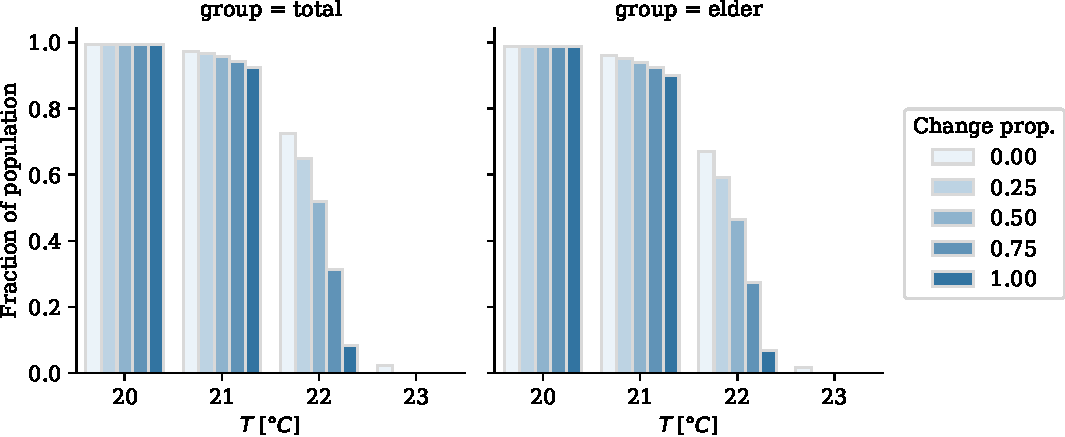
\includegraphics[width=.6\textwidth]{figures/human-exposure}
  \caption{\label{fig:human-exposure} Population exposed to temperatures higher than 21, 22, 23, 24, 25 and 26$\degree$C respectively for an overall proportion of transformed pixels of 0, 25, 50, 75 and 100\%. The bar heights and the confidence intervals are computed out of all the simulation runs and sampling approaches. See the Juptyer Notebook at \hyperref[sec:si-human-exposure]{section S2.3} for the detailed numbers of the figure.}
\end{figure}
% The number of dwellers exposed to temperatures higher than 22$\degree$C diminishes as the number of pixels transformed to high tree canopy classes increases.
% (on average over all the simulation runs and sampling approaches)
The number of dwellers exposed to temperatures higher than 21$\degree$C does not show a significant decrease (even when converting all the candidate pixels), whereas for temperatures higher than 22$\degree$C, it diminishes from 269254 to 268601, 267683, 266518 and 264125 when the proportion of transformed pixels is of 25, 50, 75 and 100\% respectively, which represents a relative share of 97.25, 97.02, 96.69 96.27 and 95.41\% of the population of the study area.
% For temperatures over 23$\degree$C, the corresponding decreases start from 254653 to 250392, 243063, 231065 and 210802, representing a 91.98 to 90.44, 87.80, 83.46 and 76.14\% of the population, while for temperatures over 24$\degree$C 217051, 200406, 164908, 103889 and 31905, respectively representing a 78.40, 72.39, 59.57, 37.53 and 11.52$\degree$C.
Such a decline progressively becomes more notable as temperatures increase, e.g., the share of the population exposed to temperatures over 24$\degree$C declines from an initial 78.4\% to 72.39, 59.57, 37.53 and 11.52\% when transforming a 25, 50, 75 and 100\% of the candidate pixels respectively.
% Finally, the number of dwellers exposed to temperatures over 25$\degree$C decreases from 132641 to 69162 and 15866 for proportions of transformed pixels of 25 and 50\% respectively, representing a 47.91, 24.98 and 5.73\% of the total population, and becomes 0 after that, whereas the totality 2508 dwellers originally exposed to temperatures over 26$\degree$C, which represents a 0.91\% of the population, do no longer meet such temperatures after transforming a 25\% of the candidate pixels.
Finally, the share of dwellers exposed to temperatures over 25$\degree$C, which is initially of 47.91\%, is diminished to a 24.98 and 5.74\% when transforming a 25 and 50\% of the pixels respectively, and becomes 0 after that, whereas the 2508 dwellers originally exposed to temperatures over 26$\degree$C do no longer meet such temperatures after transforming a 25\% of the candidate pixels.

% The differences between the spatially scattering or scattering the transformed pixels are most notable when considering the number of dwellers exposed to temperatures higher than 24$\degree$C and 25$\degree$C.
% Regarding the spatial configurations, scattering the transformed pixels instead of clustering them with other high tree canopy pixels can result in a reduction of the 3238, 9597 and 15323 dwellers exposed to temperatures higher than 24$\degree$C for the same proportions of transformed pixels of 25, 50 and 75\%, which respectively represents a 1.17, 3.47 and 5.53\% of the total number of dwellers. For temperatures higher than 25$\degree$C, the analogous reduction is of 20708 and 22748 dwellers when transforming a 25 and 50\% of the pixels, which represents a 7.48 and 8.22\% of the population.
The way in which the transformed pixels are sampled has significant effects on the human exposure to high temperatures (\autoref{fig:human-exposure-comparison}). 
\begin{figure}[ht]
  \begin{adjustwidth}{-.4\textwidth}{0cm}  
    \centering
    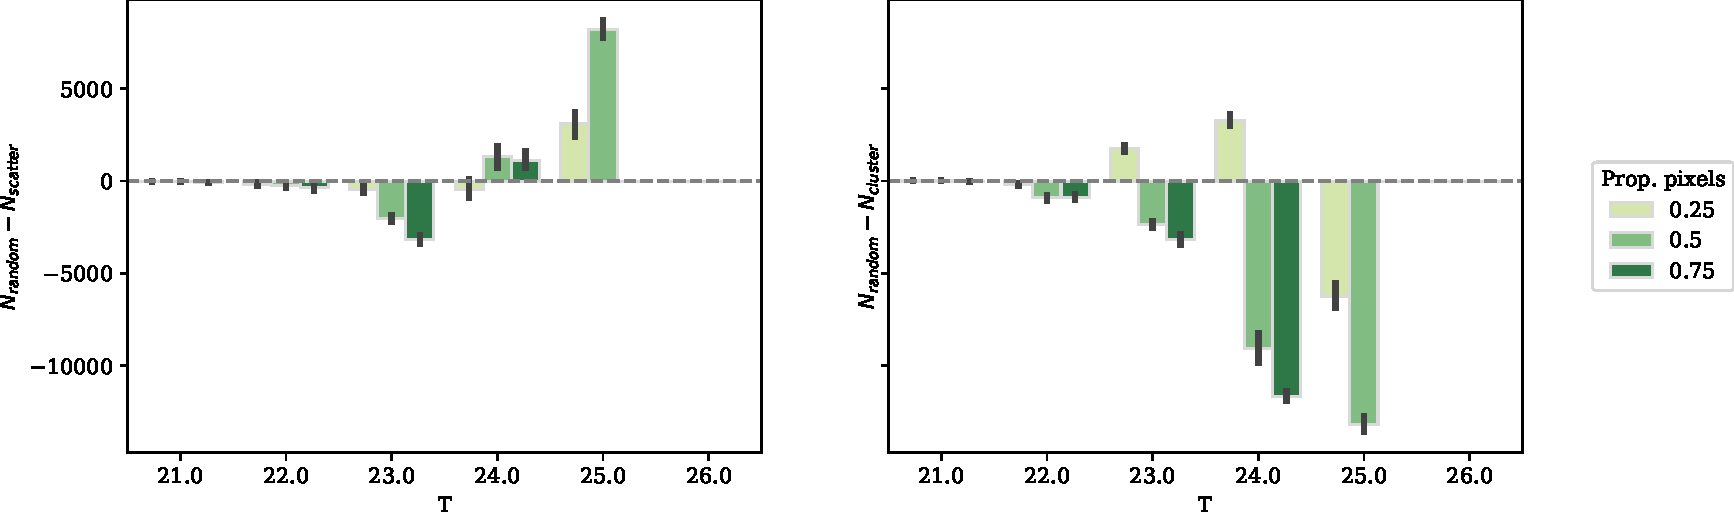
\includegraphics[width=\linewidth]{figures/human-exposure-comparison}
    \caption{\label{fig:human-exposure-comparison}
      % Effect of the sampling approach on the population exposed to temperatures higher than 21, 22, 23, 24, 25 and 26$\degree$C for an overall proportion of transformed pixels of 0, 25, 50 and 75\%.
      Comparison of between the population exposed to temperatures higher than 21, 22, 23, 24, 25 and 26$\degree$C with the random sampling approach and the scattering ($N_{random} - N_{scatter}$, left subplot) and the clustering ($N_{random} - N_{cluster}$, right subplot) selection approaches, for an overall proportion of transformed pixels of 25, 50 and 75\%.
      The lines at the top of the bars represent the 95\% confidence intervals. The bar heights and the confidence intervals are computed out of all the simulation runs. See the Jupyter Notebook at \hyperref[sec:si-human-exposure]{section S2.3} for the detailed numbers of the figure.}
  \end{adjustwidth}
\end{figure}
Overall, scattering the transformed pixels to avoid forming a continuous tree canopy appears as the most effective approach to reduce the human exposure to the highest temperatures, followed by random sampling.
When transforming a 25 and 50\% of the candidate pixels with the scattering approach, the number of dwellers exposed to temperatures over 25$\degree$C decreases from 124073 to 65108 and 4498 respectively. % (which is 4.57 an 64.57\% larger than the corresponding reduction when averaged among the three approaches)
Such a reduction is larger than its random sampling counterpart by 3125 and 8223 dwellers respectively, and larger than its clustering approach counterpart by 9359 and 21388 dwellers respectively (\autoref{fig:human-exposure-comparison}).
% which is larger than its counterpart when reduction  corresponds to  less dwellers than when transforming the same amount of pixels with random sampling approach, and 9359 and 21388.



\section*{Discussion}

% \subsection*{Complexity of the impact of the spatial pattern of tree canopy on urban heat mitigation}
\subsection*{Validity and applicability of the proposed approach}

% The scenarios simulated in this study represent a new form of exploring the heat mitigation potential provided by the urban tree canopy cover.
% The results map locations where the tree canopy cover in the urban agglomeration of Lausanne can be increased, and shows that such changes can result in urban nighttime temperatures that are up to 2$\degree$C lower.
% Additionally, the number of dwellers exposed to nighttime temperatures over 24$\degree$C can be reduced from 217051 to 31905, which respectively represents a 78.40 and 11.52\% of the total population in the study area.
The scenarios simulated in this study map locations where the tree canopy cover in the urban agglomeration of Lausanne can be increased, and suggests that such changes can result in urban nighttime temperatures that are up to 2$\degree$C lower.
% 1. EFFECTS OF THE SPATIAL CONFIGURATION
% % The proposed simulation approach presents several major advantages when compared to statistical analyses.
% Overall, the simulated scenarios in Lausanne indicate that given the same proportion of tree canopy cover, a scattered configuration might result in more effective urban heat mitigation than a clustered one, both in terms of the average temperature and the number of urban dwellers exposed to the highest tempetratures.
% % might have the spatial configuration of the tree canopy might indeed have a significant effect on the spatial pattern of air temperature, yet it seems that such an effect is very small when compared to the effect of the proportion of tree cover
% Nevertheless, the results suggest that effect of the spatial configuration is secondary when compared to the effect of the composition, i.e., proportion of tree cover.
% % Trees contribute to urban heat mitigation in two primary ways, namely the shading and evapotranspiration processes. Therefore, the effect of the spatial configuraiton of trees on its cooling effectiveness
% The effect of the spatial configuration of trees on its urban cooling effectiveness depends on how it affects the shading and evapotranspiration processes. Such a relationship is know to be highly complex and dependent on the ecological context \cite{zhou2017effects}, tree species \cite{jiao2017patch}
% The simulated scenarios in Lausanne indicate that given the same proportion of tree canopy cover, a scattered configuration might result in more effective urban heat mitigation than a clustered one, which is in line with previous studies in humid climates \cite{kong2014effects,estoque2017effects,zhou2017effects,yu2018strong,nastran2019urban}.
The results indicate that given the same proportion of tree canopy cover, a scattered configuration might lead to more effective urban heat mitigation than a clustered one, which is in line with previous studies in humid climates \cite{zhou2011does,kong2014effects,estoque2017effects,zhou2017effects,yu2018strong,nastran2019urban}.
Nevertheless, the results suggest that effect of the spatial configuration (measured by the metrics AREA\_MN, SHAPE\_MN and ED) is secondary when compared to the effect of the composition (measured by the PLAND metric).
% Overall, the effect of the spatial configuration of trees on its urban cooling effectiveness depends on how it affects the shading and evapotranspiration processes, which is known to be highly complex relationship that is strongly mediated by the tree species as well as the local climatic and environmental conditions \cite{zhou2017effects,jiao2017patch,yu2018strong,wang2020significant}. Furthermore, the cooling effects of tree canopy cover are scale-dependent \cite{li2013relationship,estoque2017effects,yan2019testing,wang2020significant,terfa2020spatial}.
% Overall, the effect of the spatial configuration of trees on its urban cooling effectiveness depends on how it affects the shading and evapotranspiration processes.
Overall, the effect of the spatial configuration of trees on its urban heat mitigation depends on how it affects the shading and evapotranspiration processes.
Such a relationship is known to be strongly mediated by the tree species, background climatic and environmental conditions as well as the spatial scale \cite{li2013relationship,estoque2017effects,zhou2017effects,jiao2017patch,yu2018strong,yan2019testing,wang2020significant,terfa2020spatial}.

% 2. NON-LINEARITIES AND THRESHOLDS
% In order to better represent the effects of the spatial configuration of the tree canopy, the InVEST urban cooling model must be further validated with experiments at the neighborhood scale to ensure that it provides an appropriate city-scale depiction of how the urban heat mitigation mechanisms operate at finer scales.
The spatial effects observed in the results are due to the InVEST model equations representing air mixing and the effect of parks. In order to ascertain these effects, the InVEST urban cooling model must be further validated with experiments at the neighborhood scale to ensure that it provides an appropriate city-scale depiction of how the urban heat mitigation mechanisms operate at finer scales.
% The proposed approach provides an effective interface to spatially evaluate mitigation strategies. Further refinement of the urban cooling model (i.e., including non-linearities) might enable further explorations (e.g., thresholds).
% Multi-scale perspective \cite{wang2020spatial}
% gains are orthogonal to those of green roofs
% We also need to compare the urban cooling model to more fine-grained models (e.g., three-dimensional models at the neighborhood scale) to find out whether the urban cooling model provides an adequate averaging of the neighborhood scale behaviour. We have the required high-resolution data for most parts (e.g., cadastre, tree canopy) but not high-resolution air temperature measurements (in space and time). Note that LST is not good enough
% While the InVEST urban cooling model provides an effective method to simulate urban heat mitigation from LULC rasters at the urban agglomeration scale \cite{bosch2020spatially}, it must be further validated with experiments at the neighborhood scale to ensure that it provides an appropriate upscale representation of how the urban heat mitigation mechanisms operate at finer scales.
% On the other hand, the InVEST urban cooling models presents limitations regarding the simplified and homogeneous way in which the air is mixed, as well as the cooling effects of large green spaces \cite{sharp2020invest,bosch2020spatially}.
In fact, the InVEST urban cooling model presents limitations regarding the simplified and homogeneous way in which the air is mixed, as well as the cooling effects of large green spaces \cite{sharp2020invest,bosch2020spatially}.
As a result, the relationship between the proportion of tree canopy cover and the magnitude of the urban heat mitigation reported in this work is practically linear, and the temperature differences between spatially clustering or scattering the new tree canopy cover are limited.
Nonetheless, in complex terrains such as the Lausanne agglomeration, models with uniform weighting of space show considerable deviations from the observed spatial patterns of air temperature \cite{frei2014interpolation,labedens2019modeling}. Moreover, the cooling effects of large green spaces have been found to be non-proportional to their area and shape complexity \cite{chen2014effect,bao2016assessing,du2017quantifying}.
% Including non-linearities of this kind may not only make the urban cooling model more realistic but also more useful for urban planning, e.g., by suggesting thresholds in the relatinship between the proportion of tree canopy cover and the simulated heat mitigation that ensure ``optimal'' spending.
Improving how these non-linear components are represented in the InVEST urban cooling model could enhance not only its validity, but also its value to urban planning by identifying thresholds and regime changes in the cooling efficiency of additional tree planting.
% MAYBE: while there is scope for improvement, the current implementation of the model suggests that there are thresholds regarding human exposure.
% MAYBE: virtual explorations: ``A concept that emerges quite naturally from such purposive bottom-up actions is the idea that to explore good planning and design in cities, computer models should be set up in a laboratory-like context in which the focus is on exploration of different patterns which attempt to reach different goals, laboratories in which models are available in wide area mode, across the web in a form that many people can experiment with.'' \cite[page 115]{batty2010complexity}, \cite{de2010planner,bosch2019addressing}


% \subsection*{Applicability of the proposed approach}

% 3. EVALUATE FUTURE SCENARIOS, COMPARE SPRAWL VS INFILL
% Additionally, we can use the approach to compare distinct urban expansion scenarios (e.g., compact, sprawl) \cite{lemonsu2015vulnerability,yang2016contrasting}, also landscape homogenization along the urban-rural gradient \cite{wang2020spatial}.
Despite the limitations noted above, a major advantage of the proposed approach is that it can be used to evaluate urban heat mitigation of synthetic scenarios.
The simulations presented in this article focus on spatially exploring the effects of an increase of the tree canopy cover, yet there is room for much more experimentation of this kind.
% For instance,
% For instance, the sampling approaches to select the transformed pixels explored above can be replaced by ad-hoc optimization procedures that aim at minimizing the exposure of the most vulnerable populations to critical heat thresholds.
On the one hand, the generic sampling approaches explored above can be extended to consider ad-hoc characteristics such as the spatial distribution of the population, and design optimization procedures with specific goals. For instance, the candidate pixels can be selected with the aim of minimizing the exposure of the most vulnerable populations to critical heat thresholds.
% The approach can be used as part of a broader decision support system to explore the trade-offs between ecosystem services provided by trees, perform weighted optimizations and map priority planting locations \cite{bodnaruk2017plant}.
More broadly, the approach can be used as part of decision support system to explore the trade-offs between ecosystem services provided by trees, perform weighted optimizations and map priority planting locations \cite{bodnaruk2017plant}.
% MAYBE: landscape ecology principals/network planning to ensure connectivity and the like? see \cite[page 766]{haaland2015challenges}
On the other hand, in line with recent studies \cite{lemonsu2015vulnerability,yang2016contrasting,trimmel2019thermal}, the approach could be applied to examine the impact of distinct urbanization scenarios such as densification and urban sprawl on air temperature and human exposure to extreme heat, under current conditions as well as future climate estimates, e.g., by changing the $T_{ref}$ or $UHI_{max}$ parameters.
Similarly, InVEST urban cooling model might be coupled with models of LULC change such as cellular automata in order to assess not only which scenarios are most desirable in terms of urban heat mitigation, but also which planning strategies might lead to them \cite{silva2008strategies,white2015modeling,bosch2019addressing}.
% Also to evaluate projected LULC maps (e.g., outputs of cellular-automata simulations \cite{bosch2019addressing})

% TODO: multi-scale \cite{artmann2019urban,wang2020spatial}, complimentary to other approaches (e.g., green roofs) and urban planning indicators

% TODO: different impacts in different cities \cite{zhou2017effects,gret2020urban}


\subsection*{Implications for urban planning in Lausanne}

The spatiotemporal patterns of LULC change observed during the last 40 years in the Lausanne agglomeration have been characterized by infilling development and a progressive coalescensce of artificial surfaces in its inner ring \cite{bosch2020spatiotemporal}.
% Overall decrease of urban green space in European cities due to infill development \cite{haaland2015challenges}.
Such an infilling trend urges for careful evaluation of the beneficial ecosystem services provided by urban green spaces, which should be balanced against the adverse consequences of urban sprawl \cite{haaland2015challenges,artmann2019urban}.

The approach proposed in this study maps locations in the current urban fabric where the tree canopy cover can be increased.
While part of this urban greening might occur in impervious surfaces (e.g., in sidewalks, next to roads and in other impervious surfaces), most of the candidate locations currently correspond to urban green space (i.e., the ``garden'' LULC class).
Therefore, the potential heat mitigation suggested by the results study is not attainable in a scenario of severe infill development.
Additionally, densification strategies should consider that newly created urban green space might result in less provision of ecosystem services than remnant natural patches \cite{jim2013sustainable,sun2017effects,wang2019quantity}.
Finally, infilling might exacerbate the unevenness of the accessibility to green areas by depriving dwellers of the most dense parts in city core from their few remaining urban green spaces.  % \cite{wolch2014urban}
% TODO: evenness of the distribution \cite{wolch2014urban}
% TODO: Spatially explicit is crucial
Spatial heterogeneity of this kind, which are encountered in many socioeconomic and environmental aspects of contemporary cities, are often hard to represent with aggregate indicators and highlight the importance of spatially explicit models to urban planning and decision making.


% TODO: human exposure, example heat wave 2003 in Switzerland \cite{grize2005heat}
The explicit representation of space is also crucial when considering the impacts of urban green space on human exposure to extreme heat.
Although the simulated scenarios suggest that the impact of the spatial pattern of tree canopy on the air temperature is practically linear, the implications on human exposure to critical temperatures exhibit important thresholds.
% For example, the number of dwellers exposed to nighttime temperatures over 24$\degree$C can be reduced from 217051 to 31905, which respectively represents a 78.40 and 11.52\% of the total population in the study area.
For example, by increasing the tree canopy cover of a 25\% of the candidate pixels, the number of dwellers exposed to nighttime temperatures over 25$\degree$C can be reduced from 124073 to 74466, which respectively represents a 45.08 and 27.06\% of the total population in the study area.
Furthermore, the results suggest by selecting such pixels to prioritize a spatial scattering of the tree canopy cover, such a population can be reduced by an additional 3125 or 6234 dwellers when respectively compared to random sampling such pixels or clustering them to the existing tree canopy cover.
In Switzerland, the excess mortality associated to the heat wave of 2003 occurred over-proportionally to urban and sub-urban residents of its largest urban agglomerations \cite{grize2005heat}.
% TODO: relationship between heat and mortality in Switzerland \cite{ragettli2017exploring}
Furthermore, the association between temperature and mortality in extreme heat events in the largest Swiss urban agglomerations are exponential \cite{ragettli2017exploring}, which indicates that reducing temperatures by even fractions of a degree can have a dramatic impact on death rates.



\section*{Conclusion}
% TODO: conclusions
The scenarios simulated in this study represent a new way of spatially exploring the heat mitigation potential provided by modifications of the urban fabric, and allow evaluating the cooling effects of both the abundance and spatial configuration of the tree canopy cover.
The results map locations where the existing tree canopy cover of the urban agglomeration of Lausanne can be increased, and show an urban cooling potential for urban nighttime temperatures of more than 2$\degree$C.
% Additionally, the number of dwellers exposed to nighttime temperatures over 24$\degree$C can be reduced from 217051 to 31905, which respectively represents a 78.40 and 11.52\% of the total population in the study area. ALSO SCATTERING
Additionally, the simulations suggest that the spatial configuration in which the tree canopy is increased influences its heat mitigation effects.
The configuration effects become more significant when considering the impacts on the urban population, and small increases in the tree canopy can result in important reductions in the number of dwellers exposed to the highest temperatures.
Overall, the presented approach provides a novel way to explore how the urban tree canopy can be exploited to reduce heat stress.
Future studies can extend the analyses by assessing the provision of other ecosystem services in the various tree canopy strategies presented here.


\section*{Supporting Information}

%These commands reset the figure/table counter and add "S" to the figure/table caption (e.g. "Figure S1"/"Table S1").
\setcounter{figure}{0}
\renewcommand{\thefigure}{S\arabic{figure}}
\setcounter{table}{0}
\renewcommand{\thetable}{S\arabic{table}}

\section*{S1 Data}

\subsection*{S1.1 Biophysical table}
\label{sec:si-biophysical-table}

% Biophysical table (before the reclassification), as comma-separated values (CSV).
% \url{https://github.com/martibosch/lausanne-heat-islands/blob/master/data/raw/biophysical-table.csv}
The biophysical table for the LULC codes (before the reclassification) is shown in \autoref{tab:si-biophysical-table}. The crop and water coefficients are based on Allen et al. \cite{allen1998crop}, while rock, soil and urban coefficients are derived from the results of Grimmond and Oke \cite{grimmond1999evapotranspiration} in the city of Chicago. Given that the evapotranspiration of the vegetation and crops is subject to seasonal changes in temperate zones such as Switzerland \cite{allen1998crop}, the values that correspond to the mid-season estimation (June to August) in \cite{nistor2016mapping}.
The albedo values are based on the work of Steward et al. \cite{stewart2012local}.
The shade column, which represents the proportion of tree cover of each LULC class, is computed after the reclassification procedure described in section ``\nameref{sec:refin-lulc-class}''. % \autoref{sec:refin-lulc-class}.

\begin{table}[!h]
  \begin{adjustwidth}{-.1\textwidth}{0cm}
    \caption{\label{tab:si-biophysical-table} Biophysical table (before the reclassification). The source comma-separated value (CSV) file used in the computational workflow is available at \url{https://github.com/martibosch/lausanne-heat-islands/blob/master/data/raw/biophysical-table.csv}.}
    \begin{center}
      \begin{tabular}{ c p{.28\textwidth} p{.16\textwidth} c c c }
        \toprule
        LULC code & Description & Case & $K_c$ & Albedo & Green area \\
        \midrule
        0 & building & artificial & 0.4 & 0.1-0.25 & 0 \\ % 0.142
        1 & road, path & artificial & 0.35 & 0.15 & 0 \\ % 0.141
        2 & sidewalk & artificial & 0.35 & 0.15 & 0 \\
        3 & traffic island & artificial & 0.35 & 0.15 & 0 \\
        4 & rail & artificial & 0.35 & 0.15 & 0 \\
        5 & airfield & artificial & 0.4 & 0.2 & 0 \\
        6 & pond & water & 0.45 & 0.15 & 0 \\
        7 & other impervious & artificial & 0.36 & 0.15 & 0 \\
        8 & field, meadow, pasture & vegetation & 0.9 & 0.2 & 1 \\
        9 & vineyards & vegetation & 0.7 & 0.2 & 1 \\
        10 & other intensive farming & vegetation & 1.05 & 0.2 & 1 \\
        11 & garden & artificial & 0.32 & 0.2 & 1 \\
        12 & wetland & water & 0.45 & 0.1 & 1 \\
        13 & other green & vegetation & 0.45 & 0.2 & 1 \\
        14 & backwater & water & 0.65 & 0.05 & 1 \\
        15 & water course & water & 0.65 & 0.05 & 0\\
        16 & reed & water & 0.45 & 0.1 & 1\\
        17 & dense forest & vegetation & 1.5 & 0.15 & 1 \\
        18 & densely wooded pasture & vegetation & 1.15 & 0.15 & 1 \\
        19 & open wooded pasture & vegetation & 1.15 & 0.2 & 1 \\
        20 & other wooded & vegetation & 1.15 & 0.15 & 1\\
        21 & bare rocks & rock and soil & 0.2 & 0.25 & 0 \\
        22 & glacier & water & 0.52 & 0.1 & 0 \\
        23 & sand & rock and soil & 0.3 & 0.25 & 0 \\
        24 & gravel pit & artificial & 0.36 & 0.25 & 0 \\
        25 & other non-vegetated & artificial & 0.36 & 0.15 & 0 \\
        \bottomrule
      \end{tabular}
      % \caption{\label{tab:evapotranspiration-coefficients}
      % Evapotranspiration coefficients for each LULC class (see \nameref{table-biophysical}). Crop and water coefficients are based on Allen et al. \cite{allen1998crop}, while rock, soil and urban coefficients are derived from the results of Grimmond and Oke \cite{grimmond1999evapotranspiration} in the city of Chicago. Given that the evapotranspiration of the vegetation and crops is subject to seasonal changes in temperate zones such as Switzerland \cite{allen1998crop}, the values that correspond to the mid-season estimation (June to August) in \cite{nistor2016mapping}.
      % The albedo values are based on the work of Steward et al. \cite{stewart2012local}.
      % The source comma-separated value (CSV) file used in the computational workflow is available at \url{https://github.com/martibosch/lausanne-heat-islands/blob/master/data/raw/biophysical-table.csv}.
      % }
    \end{center}
    % \vspace{.5em}
    % \textbf{Table S3.} Biophysical table. The crop and water coefficients are based on Allen et al. \cite{allen1998crop}, while rock, soil and urban coefficients are derived from the results of Grimmond and Oke \cite{grimmond1999evapotranspiration} in the city of Chicago. Given that the evapotranspiration of the vegetation and crops is subject to seasonal changes in temperate zones such as Switzerland \cite{allen1998crop}, the values that correspond to the mid-season estimation (June to August) in \cite{nistor2016mapping}.
    % The albedo values are based on the work of Steward et al. \cite{stewart2012local}.
    % The source comma-separated value (CSV) file used in the computational workflow is available at \url{https://github.com/martibosch/lausanne-heat-islands/blob/master/data/raw/biophysical-table.csv}.
  \end{adjustwidth}
\end{table}


% \section{Relationships between the spatial patterns of tree canopy and air temperature}
% \label{sec:spatial-relationships}

% Exploration of relationships between the spatial patterns of tree canopy and air temperature, as Jupyter Notebook (IPYNB) \url{https://github.com/martibosch/lausanne-greening-scenarios/blob/master/notebooks/spatial-relationships.ipynb}.

\subsection*{S1.2 Monitoring stations}
\label{sec:monitoring-stations}

The locations of the monitoring stations used to get the $T_{ref}$ and $UHI_{max}$ parameters of the InVEST urban cooling model are shown in \autoref{fig:monitoring-stations}. The operators of the stations are: Agrometeo, Federal roads office (ASTRA), Federal office for the environment (BAFU), General directorate for the environment of the Canton of Vaud (DGE), and the Federal Institute of Forest, Snow and Landscape Research (WSL) \cite{rebetez2018meteorological}.
The source CSV file with the operator, location and elevation in meters above sea level of the monitoring stations used in the computational workflow is available at \url{https://github.com/martibosch/lausanne-greening-scenarios/blob/master/data/raw/tair-stations/station-locations.csv}.
The code to produce \autoref{fig:monitoring-stations} is available as a Jupyter Notebook (IPYNB) at \url{https://github.com/martibosch/lausanne-greening-scenarios/blob/master/notebooks/stations.ipynb}.

\begin{figure}[H]
  \centering
  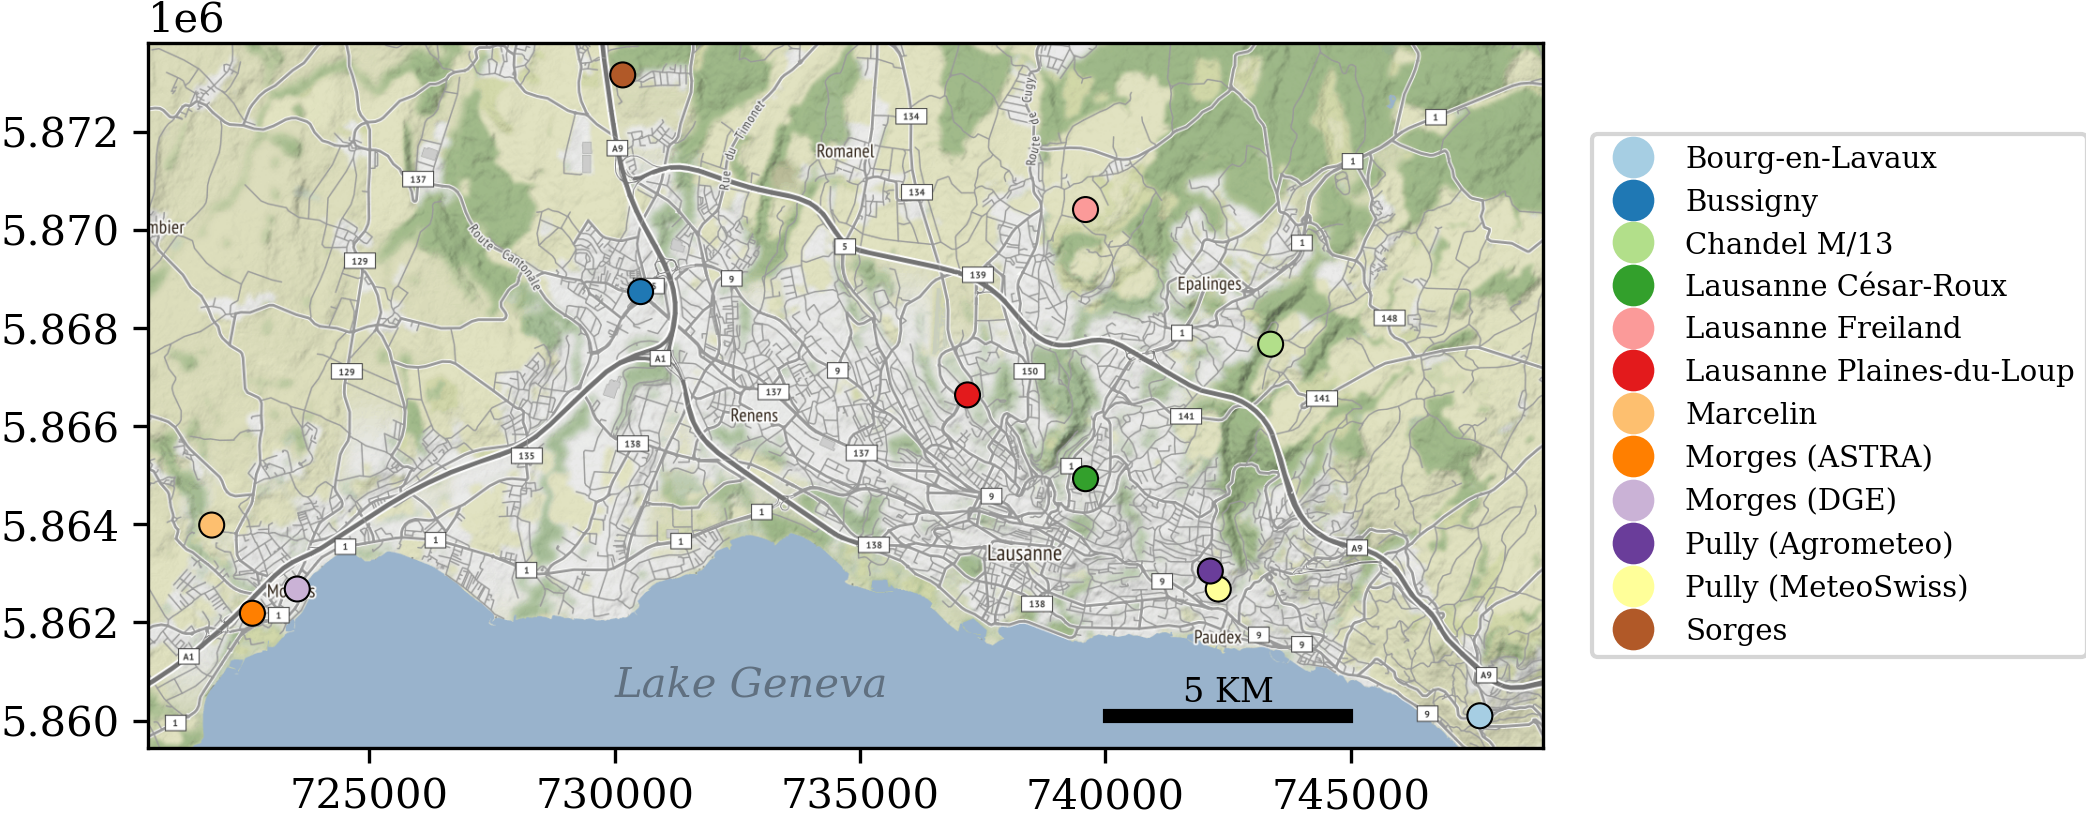
\includegraphics[width=.98\textwidth]{figures/monitoring-stations}
  \caption{\label{fig:monitoring-stations} Locations of the monitoring stations used to get the $T_{ref}$ and $UHI_{max}$ parameters. The axes tick labels display the Swiss CH1903+/LV95 coordinates. The basemap tile is provided by StamenDesign, under CC BY 3.0, with data from OpenStreetMap, under ODbL.}
\end{figure}


\section*{S2 Results}

% \subsection*{Effect of the sampling approach on LULC change}
% \label{sec:effect-approach-lulc}

% \begin{figure}
%   \begin{adjustwidth}{-.4\textwidth}{0cm}  
%     \centering
%     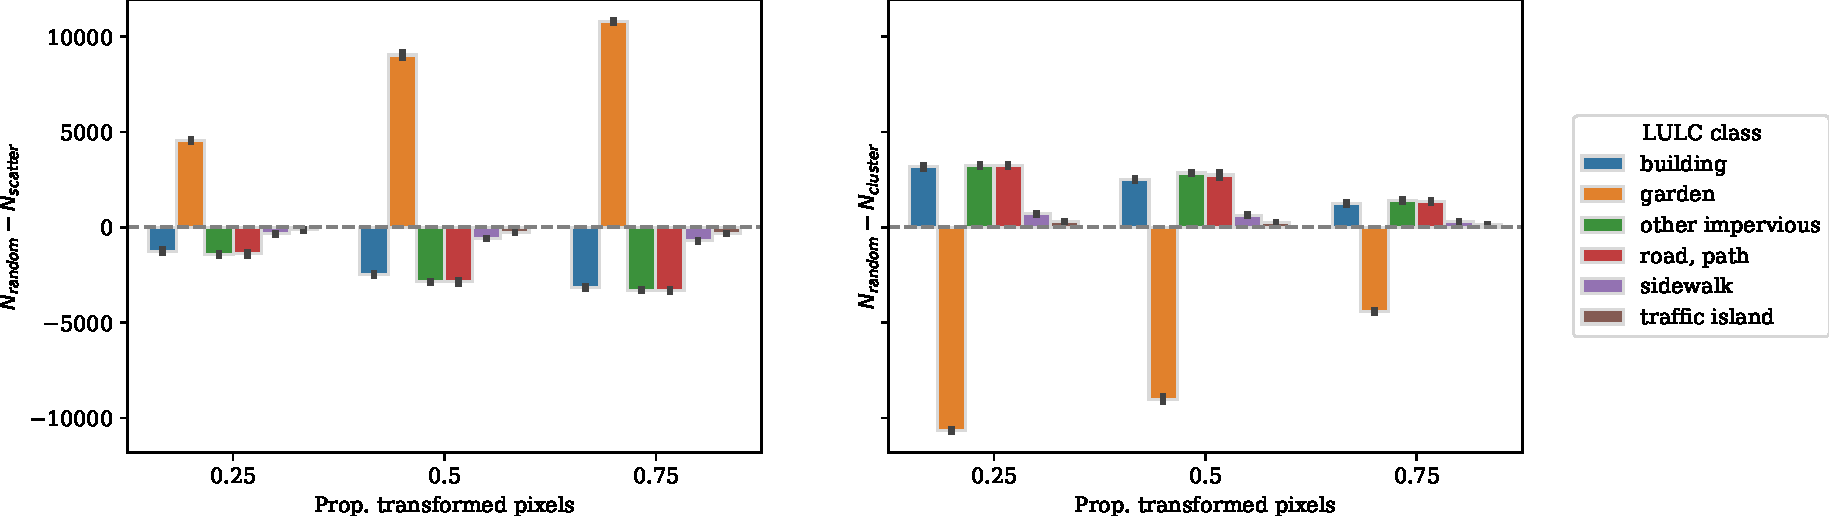
\includegraphics[width=\linewidth]{figures/scenario-lulc-barplot-comparison}
%     \caption{\label{fig:scenario-lulc-barplot-comparison} Effect of the sampling approach on LULC change}
%   \end{adjustwidth}
% \end{figure}

\subsection*{S2.1 Scenario LULC, temperature and heat mitigation}
\label{sec:si-scenarios}

% The code for the evaluation of scenarios generated to explore the effect of increasing the proportion of tree cover
The code to produce the figures \ref{fig:scenario-lulc-barplot}, \ref{fig:scenario-maps}, \ref{fig:si-scenario-T-regplot} and \ref{fig:si-scenario-T-hists}, as well as tables describing the data of the figures, are available as a Jupyter Notebook (IPYNB) at \url{https://github.com/martibosch/lausanne-greening-scenarios/blob/master/notebooks/scenarios.ipynb}.

\begin{figure}[H]
  \centering
  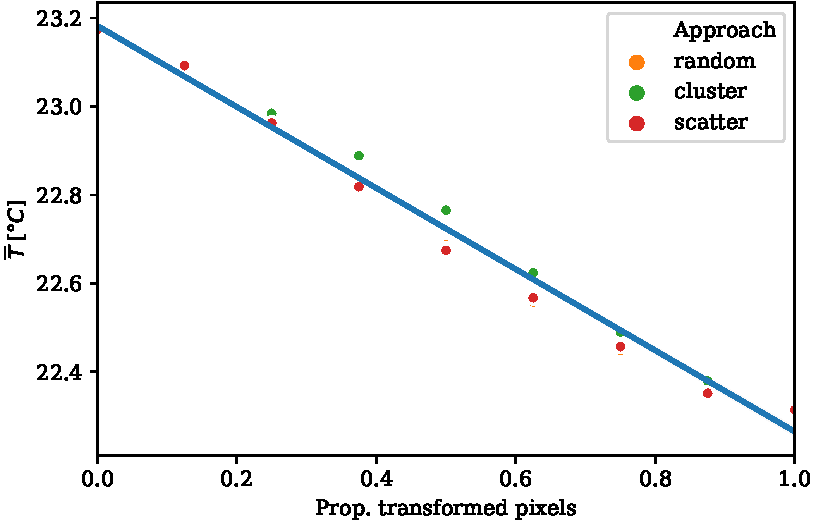
\includegraphics[width=.6\textwidth]{figures/scenario-T-regplot}
  \caption{\label{fig:si-scenario-T-regplot} Relationship between the proportion of candidate pixels transformed and the average simulated temperature $\overline{T}$ for each scenario sample. The translucent bands around the regression line represent the 95\% confidence intervals estimated using a bootstrap.}
\end{figure}


\begin{figure}[H]
  \centering
  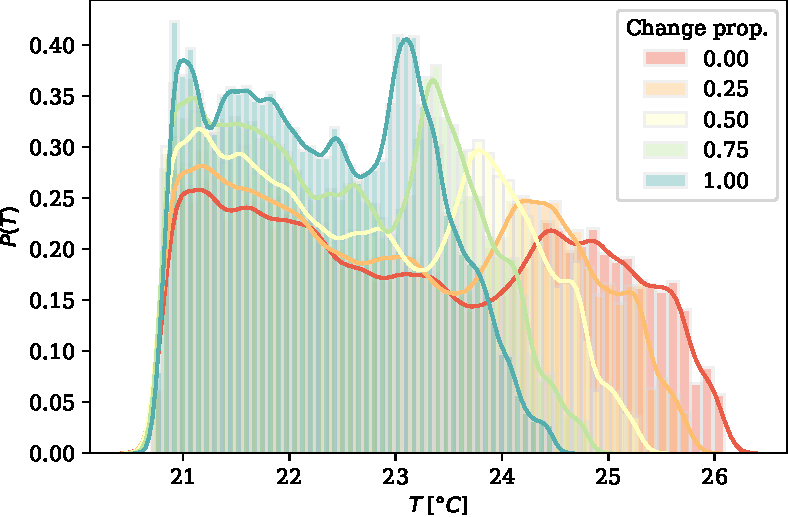
\includegraphics[width=.6\textwidth]{figures/scenario-T-hists}
  \caption{\label{fig:si-scenario-T-hists} Histogram of raster temperature values for a 25, 50, 75 and 100\% of the candidate pixels transformed. The temperature rasters for each histogram are computed by averaging the 10 simulations with the same proportion of candidate pixels transformed.}
\end{figure}


\subsection*{S2.2 Scenario metrics}
\label{sec:si-scenario-metrics}

% Evaluation of scenarios generated to explore the effect of the spatial configuration of tree cover, as Jupyter Notebook (IPYNB) \url{https://github.com/martibosch/lausanne-greening-scenarios/blob/master/notebooks/scenarios-config.ipynb}.
The code to produce \autoref{fig:scenario-metrics} is available as a Jupyter Notebook (IPYNB) at \url{https://github.com/martibosch/lausanne-greening-scenarios/blob/master/notebooks/scenario-metrics.ipynb}.


\subsection*{S2.3 Scenario human exposure}
\label{sec:si-human-exposure}

% Evaluation of scenarios generated to explore the effect of the spatial configuration of tree cover, as Jupyter Notebook (IPYNB) \url{https://github.com/martibosch/lausanne-greening-scenarios/blob/master/notebooks/human-exposure.ipynb}.

The code to produce \autoref{fig:human-exposure} is available as a Jupyter Notebook (IPYNB) at \url{https://github.com/martibosch/lausanne-greening-scenarios/blob/master/notebooks/human-exposure.ipynb}.

\section*{Acknowledgments}
This research has been supported by the \'Ecole Polytechnique F\'ed\'erale de Lausanne (EPFL).

\nolinenumbers

% This is where your bibliography is generated. Make sure that your .bib file is actually called library.bib
\bibliography{references}

%This defines the bibliographies style. Search online for a list of available styles.
\bibliographystyle{unsrt}

\end{document}
